\subsection{Oscillation equations test}

Let us consider the \emph{oscillation} problem, it being a simple, yet interesting IVP. Briefly, the oscillation problem is a prototype problem of non dissipative, oscillatory phenomena. For example, let us consider a pendulum subjected to the Coriolis accelerations without dissipation, the motion equations of which can be described by the ODE system \ref{eq:oscillation}.

\begin{equation}
\begin{matrix}
U_t = R(U)  \\
U = \begin{bmatrix}
x \\
y
\end{bmatrix}\;\;\;
R(U) = \begin{bmatrix}
-f y \\
f x
\end{bmatrix}
\end{matrix}
\label{eq:oscillation}
\end{equation}
where the frequency is chosen as $f=10^4$. The ODE system \ref{eq:oscillation} is completed by the following initial conditions:

\begin{equation}
\begin{matrix}
  x(t_0) = 0 \\
  y(t_0) = 1
\end{matrix}
\label{eq:oscillation-ic}
\end{equation}
where $t_0=0$ is the initial time considered.

The IVP constituted by equations \ref{eq:oscillation} and \ref{eq:oscillation-ic} is (apparently) simple and its exact solution is known:

\begin{equation}
\begin{matrix}
  x(t_0 + \Delta t) = X_0 cos(f \Delta t) - y_0 sin(f \Delta t) \\
  y(t_0 + \Delta t) = X_0 sin(f \Delta t) + y_0 cos(f \Delta t)
\end{matrix}
\label{eq:oscillation-exact}
\end{equation}
where $\Delta t$ is an arbitrary time step. This problem is non-stiff meaning that the solution is constituted by only one time-scale, namely the single frequency $f$.

This problem is only apparently simple. As a matter of facts, in a non dissipative oscillatory problem the eventual errors in the amplitude approximation can rapidly drive the subsequent series of approximations to an unphysical solution. This is of particular relevance if the solution (that is numerically approximated) constitutes a \emph{prediction} far from the initial conditions, that is the common case in weather forecasting.

Because the Oscillation system \ref{eq:oscillation} posses a closed exact solution, the discussion on this test has twofolds aims: to assess the accuracy of the FOODIE's built-in solvers comparing the numerical solutions with the exact one and to demonstrate how it is simple to solve this prototypical problem by means of FOODIE.

\subsubsection{Errors Analysis}

For the analysis of the accuracy of each solver, we have integrated the Oscillation equations \ref{eq:oscillation} with different, decreasing time steps in the range $[5000, 2500, 1250, 625, 320, 100]$. The error is estimated by the L2 norm of the difference between the exact ($U_e$) and the numerical ($U_{\Delta t}$) solutions for each time step:

\begin{equation}
  \varepsilon (\Delta t) = || U_e - U_{\Delta t} ||_2 = \sqrt{ \sum_{s=1}^{N_s} { \left(U_e(t_0 + s * \Delta t) - U_{\Delta t}(t_0 + s * \Delta t) \right)^2 }}
\label{eq:oscillation-error}
\end{equation}
where $N_s$ is the total number of time steps performed to reach the final integration time.

Using two pairs of subsequent-decreasing time steps solution is possible to estimate the order of accuracy of the solver employed computing the \emph{observed order} of accuracy:

\begin{equation}
  p = \frac{log10 \left( \frac{\varepsilon (\Delta t_1)}{\varepsilon (\Delta t_2)} \right)}{log10 \left( \frac{\Delta t_1}{\Delta t_2} \right)}
\label{eq:oscillation-observed-order}
\end{equation}

where $\frac{\Delta t_1}{\Delta t_2}>1$.

\subsubsection{FOODiE aware implementation of an oscillation numerical solver}

The IVP \ref{eq:oscillation} can be easily solved by means of FOODiE library. The first block of a FOODiE aware solution consists to define an \emph{oscillation integrand field} defining a concrete extension of the FOODiE \emph{integrand} type. Listing \ref{list:oscillation_type} reports the implementation of such an integrand field that is contained into the tests suite shipped within the FOODiE library.

\begin{lstlisting}[firstnumber=1,style=code,caption={implementation of the \emph{oscillation integrand} type},label={list:oscillation_type}]
type, extends(integrand) :: oscillation
  private
  integer(I_P)                           :: dims=0   ! Space dimensions.
  real(R_P)                              :: f=0._R_P ! Oscillation frequency (Hz).
  real(R_P), dimension(:),   allocatable :: U        ! Integrand (state) variables, [1:dims].
  contains
    ! auxiliary methods
    procedure, pass(self), public :: init
    procedure, pass(self), public :: output
    ! type\_integrand deferred methods
    procedure, pass(self), public :: t => dOscillation_dt
    procedure, pass(lhs),  public :: integrand_multiply_integrand => &
                                     oscillation_multiply_oscillation
    procedure, pass(lhs),  public :: integrand_multiply_real => oscillation_multiply_real
    procedure, pass(rhs),  public :: real_multiply_integrand => real_multiply_oscillation
    procedure, pass(lhs),  public :: add => add_oscillation
    procedure, pass(lhs),  public :: sub => sub_oscillation
    procedure, pass(lhs),  public :: assign_integrand => oscillation_assign_oscillation
    procedure, pass(lhs),  public :: assign_real => oscillation_assign_real
endtype oscillation
\end{lstlisting}

The \emph{oscillation} field extends the \emph{integrand} ADT making it a concrete type. This derived type is very simple: it has 5 data members for storing the state vector and some auxiliary variables, and it implements all the deferred methods necessary for defining a valid concrete extension of the \emph{integrand} ADT (plus 2 auxiliary methods that are not relevant for our discussion). The key point is here constituted by the implementation of the deferred methods: the \emph{integrand} ADT does not impose any structure for the data members, that are consequently free to be customized by the client code. In this example the data members have a very simple, clean and concise structure:
\begin{itemize}
  \item $dims$ is the number of space dimensions; in the case of equation \ref{eq:oscillation} we have $dims=2$, however the test implementation has been kept more general parametrizing this dimension in order to easily allow future modification of the test-program itself;
  \item $f$ stores the frequency of the oscillatory problem solved, that is here set to $10^{4}$, but it can be changed at runtime in the test-program;
  \item $U$ is the state vector corresponding directly to the state vector of equation \ref{eq:oscillation};
  \end{itemize}

As the listing \ref{list:oscillation_type} shows, the FOODiE implementation strictly corresponds to the mathematical formulation embracing all the relevant mathematical aspects into one derived type, a single \emph{object}. Here we not review the implementation of all deferred methods, this being out of the scope of the present work: the interested reader can see the tests suite sources shipped within the FOODiE library. However, some of these methods are relevant for our discussion, thus they are reviewed.

\paragraph{dOscillation\_dt, the oscillation residuals function}

Probably, the most important methods for an IVP solver is the residuals function. As a matter of facts, the ODE equations are implemented into the residuals function. However, the FOODiE ADT strongly alleviates the subtle problems that could arise when the ODE solver is hard-implemented within the specific ODE equations. As a matter of facts, the \emph{integrand} ADT specifies the precise interface the residuals function must have: if the client code implements a compliant interface, the FOODiE solvers will work as expected, reducing the possible errors location into the ODE equations, having designed the solvers on the ADT and not on the concrete type.

\begin{lstlisting}[firstnumber=1,style=code,caption={implementation of the \emph{oscillation integrand} residuals function},label={list:oscillation_t}]
function dOscillation_dt(self, t) result(dState_dt)
class(oscillation),     intent(IN) :: self      ! Oscillation field.
real(R_P),    optional, intent(IN) :: t         ! Time.
class(integrand),  allocatable     :: dState_dt ! Oscillation field time derivative.
integer(I_P)                       :: dn        ! Time level, dummy variable.
allocate(oscillation :: dState_dt)
select type(dState_dt)
class is(oscillation)
  dState_dt = self
  dState_dt%U(1) = -self%f * self%U(2)
  dState_dt%U(2) =  self%f * self%U(1)
endselect
return
endfunction dOscillation_dt
\end{lstlisting}

Listing \ref{list:oscillation_t} reports the implementation of the oscillation residuals function: it is very clear and concise. Moreover, comparing this listing with the equation \ref{eq:oscillation} the close correspondence between the mathematical formulation and Fortran implementation is evident.

\paragraph{add method, an example of oscillation symmetric operator}

As a prototype of the operators overloading let us consider the \emph{add} operator, it being a prototype of symmetric operators, the implementation of which is presented in listing \ref{list:oscillation_add}.

\begin{lstlisting}[firstnumber=1,style=code,caption={implementation of the \emph{oscillation integrand} add operator},label={list:oscillation_add}]
function add_oscillation(lhs, rhs) result(opr)
class(oscillation), intent(IN) :: lhs ! Left hand side.
class(integrand),   intent(IN) :: rhs ! Right hand side.
class(integrand), allocatable  :: opr ! Operator result.
allocate(oscillation :: opr)
select type(opr)
class is(oscillation)
  opr = lhs
  select type(rhs)
  class is (oscillation)
    opr%U = lhs%U + rhs%U
  endselect
endselect
return
endfunction add_Oscillation
\end{lstlisting}
It is very simple and clear: firstly all the auxiliary data are copied into the operator result, then the state vector of the result is populated with the addiction between the state vectors of the left-hand-side and right-hand-side. This is very intuitive from the mathematical point of view and it helps to reduce implementation errors. Similar implementations are possible for all the other operators necessary to define a valid \emph{intregrand} ADT concrete extension.

\paragraph{assignment of an oscillation object}

The assignment overloading of the \emph{oscillation} type is the last key-method that enforces the conciseness of the FOODiE aware implementation. Listing \ref{list:oscillation_assign} reports the implementation of the assignment overloading. Essentially, to all the data members of the left-hand-side are assigned the values of the corresponding right-hand-side. Notably, for the assignment of the state vector and of the previous time steps solution array we take advantage of the automatic re-allocation of the left-hand-side variables when they are not allocated or allocated differently from the right-hand-side, that is a Fortran 2003 feature. In spite its simplicity, the assignment overloading is a key-method enabling the usage of FOODiE solver: effectively, the assignment between two \emph{integrand} ADT variables is ubiquitous into the solvers implementations, see equation \ref{eq:RK} for example.

\begin{lstlisting}[firstnumber=1,style=code,caption={implementation of the \emph{oscillation integrand} assignment},label={list:oscillation_assign}]
subroutine oscillation_assign_oscillation(lhs, rhs)
class(oscillation), intent(INOUT) :: lhs ! Left hand side.
class(integrand),   intent(IN)    :: rhs ! Right hand side.
select type(rhs)
class is (oscillation)
  lhs%dims = rhs%dims
  lhs%f = rhs%f
  if (allocated(rhs%U)) lhs%U = rhs%U
endselect
return
endsubroutine oscillation_assign_oscillation
\end{lstlisting}

\paragraph{FOODiE numerical integration}

Using the above discussed \emph{oscillation} type it is very easy to solve IVP \ref{eq:oscillation} by means of FOODiE library. Listing \ref{list:oscillation_leapfrog} presents the numerical integration of system \ref{eq:oscillation} by means of the Leapfrog RAW-filtered method. In the example, the integration is performed with $10^4$ steps with a fixed $\Delta t=10^2$ until the time $t=10^6$ is reached. The example shows also that for starting a multi-step scheme such as the Leapfrog one a lower-oder or equivalent order one-scheme is necessary: in the example the first 2 steps are computed by means of one-step TVD/SSP Runge-Kutta 2-stages schemes. Note that the memory registers for storing the Runge-Kutta stages and the RAW filter displacement must be handled by the client code. Listing \ref{list:oscillation_leapfrog} demonstrates how it is simple, clear and concise to solve a IVP by FOODiE solvers. Moreover, it proves how it is simple and effective to apply different solvers in a coupled algorithm, that greatly simplify the development of new hybrid solvers for self-adaptive time step size.

\begin{lstlisting}[firstnumber=1,style=code,caption={numerical integration of the \emph{oscillation} system by means of Leapfrog RAW-filtered method},label={list:oscillation_leapfrog}]
use foodie, only: leapfrog_integrator, tvd_runge_kutta_integrator
type(leapfrog_integrator)        :: lf_integrator ! Leapfrog integrator.
type(tvd_runge_kutta_integrator) :: rk_integrator ! Runge-Kutta integrator.
type(oscillation)                :: rk_stage(1:2) ! Runge-Kutta stages.
type(oscillation)                :: previous(1:2) ! Previous time steps solution.
type(oscillation)                :: oscillator    ! Oscillation field.
type(oscillation)                :: filter        ! Filter displacement.
integer                          :: step          ! Time steps counter.
real                             :: Dt            ! Time step.
call lf_integrator%init()
call rk_integrator%init(stages=2)
call oscillator%init(initial_state=[0.0,1.0], f=10e4, steps=2)
Dt = 100.0
do step=1, 10000
  if (2>=step) then
    call rk_integrator%integrate(U=oscillator, stage=rk_stage, Dt=Dt, t=step*Dt)
    previous(step) = oscillator
  else
    call lf_integrator%integrate(U=oscillator, previous=previous, filter=filter, Dt=Dt, &
                                 t=step*Dt)
  endif
enddo
call print_results(U=oscillator)
\end{lstlisting}
  


\subsubsection{Adams-Bashforth}

Table \ref{tab:oscillation_errors_ab} summarizes the Adams-Bashforth error analysis. As expected, the Adams-Bashforth 1 step solution, that reverts back to the explicit forward Euler one, is unstable for all the $\Delta t$ exercised.

The expected observed orders of accuracy for the Adams-Bashforth solvers using 2, 3 and 4 time steps tend to 1.5, 2.5 and 3.5 that are in agreement with the expected formal order of 2, 3 and 4, respectively. Comparing the errors of the finest time resolution, i.e. $\Delta t=100$, we find that the L2 norm decreases of the 2 orders of magnitude as the solver's accuracy increases by 1 order. This also means that fixing a tolerance on the errors, the higher is the solver's accuracy the larger is the time resolution available. As an example, assuming that admissible errors are of $O(10^{-2})$ with the 4-steps solver we can use $\Delta t=625$ performing $N_s=t_final/625$ numerical integration steps, whereas using a 3-steps solvers we must adopt $\Delta t=100$ performing $6.25 \times N_s$ numerical integration steps instead of $N_s$. Considering that the computational costs is only slightly affected by the number of previous time steps considered\footnote{Recalling equation \ref{eq:AB} one can observe that there is only one new evaluation of the residuals function $R$ independently of the previous time steps considered. Thus, the computational costs is affected only by the increasing number of residuals summations, the costs of which are typically negligible with respect the cost of $R$ evaluation.}, the accuracy order has strong impact on the overall numerical efficiency: to improve the numerical efficiency reducing the computational costs, the usage of high order Adams-Bashforth solvers with larger time steps should be preferred instead of low order solvers with smaller time steps.

\begin{table}[!ht]
  \centering
  \caption{Oscillation test: errors analysis of explicit Adams-Bashforth solvers}\label{tab:oscillation_errors_ab}
  \begin{subtable}[b]{0.40\textwidth}
    \centering
    \caption{1 step}\label{tab:oscillation-ab-1}
    \resizebox{1.00\textwidth}{!}{%
    \begin{tabular}{ccccc}
      \toprule
      {\sc Time Step} & {\sc Error X} & {\sc Error Y} & {\sc Order X} & {\sc Order Y} \\
      \hline
      5000.0          &  0.840E+10    &  0.706E+10    & /             & /             \\
      2500.0          &  0.503E+06    &  0.570E+06    & 14.03         & 13.60         \\
      1250.0          &  0.289E+04    &  0.272E+04    &  7.45         &  7.71         \\
       625.0          &  0.239E+03    &  0.232E+03    &  3.59         &  3.55         \\
       320.0          &  0.737E+02    &  0.722E+02    &  1.76         &  1.74         \\
       100.0          &  0.250E+02    &  0.247E+02    &  0.93         &  0.92         \\
      \bottomrule
    \end{tabular}}
  \end{subtable}\quad%
  \begin{subtable}[b]{0.40\textwidth}
    \centering
    \caption{2 steps}\label{tab:oscillation-ab-2}
    \resizebox{1.00\textwidth}{!}{%
    \begin{tabular}{ccccc}
      \toprule
      {\sc Time Step} & {\sc Error X} & {\sc Error Y} & {\sc Order X} & {\sc Order Y} \\
      \hline
      5000.0          &  0.596E+03    &  0.583E+03    & /             & /             \\
      2500.0          &  0.221E+02    &  0.218E+02    & 4.75          & 4.74          \\
      1250.0          &  0.764E+01    &  0.769E+01    & 1.53          & 1.50          \\
       625.0          &  0.265E+01    &  0.268E+01    & 1.53          & 1.52          \\
       320.0          &  0.968E+00    &  0.981E+00    & 1.51          & 1.50          \\
       100.0          &  0.169E+00    &  0.171E+00    & 1.50          & 1.50          \\
      \bottomrule
    \end{tabular}}
  \end{subtable}\\
  \begin{subtable}[b]{0.40\textwidth}
    \centering
    \caption{3 steps}\label{tab:oscillation-ab-3}
    \resizebox{1.00\textwidth}{!}{%
    \begin{tabular}{ccccc}
      \toprule
      {\sc Time Step} & {\sc Error X} & {\sc Error Y} & {\sc Order X} & {\sc Order Y} \\
      \hline
      5000.0          &  0.857E+01    &  0.854E+01    & /             & /             \\
      2500.0          &  0.391E+01    &  0.386E+01    & 1.13          & 1.14          \\
      1250.0          &  0.825E+00    &  0.814E+00    & 2.24          & 2.25          \\
       625.0          &  0.150E+00    &  0.148E+00    & 2.46          & 2.46          \\
       320.0          &  0.282E-01    &  0.278E-01    & 2.49          & 2.49          \\
       100.0          &  0.154E-02    &  0.152E-02    & 2.50          & 2.50          \\
      \bottomrule
    \end{tabular}}
  \end{subtable}\quad%
  \begin{subtable}[b]{0.40\textwidth}
    \centering
    \caption{4 steps}\label{tab:oscillation-ab-4}
    \resizebox{1.00\textwidth}{!}{%
    \begin{tabular}{ccccc}
      \toprule
      {\sc Time Step} & {\sc Error X} & {\sc Error Y} & {\sc Order X} & {\sc Order Y} \\
      \hline
      5000.0          &  0.128E+07    &  0.143E+07    & /             & /             \\
      2500.0          &  0.106E+01    &  0.107E+01    & 20.21         & 20.34         \\
      1250.0          &  0.967E-01    &  0.981E-01    &  3.45         &  3.45         \\
       625.0          &  0.859E-02    &  0.871E-02    &  3.49         &  3.49         \\
       320.0          &  0.827E-03    &  0.838E-03    &  3.50         &  3.50         \\
       100.0          &  0.141E-04    &  0.143E-04    &  3.50         &  3.50         \\
      \bottomrule
    \end{tabular}}
  \end{subtable}\\
\end{table}

Figure \ref{fig:results-oscillation-adams-bashforth} shows, for each solver exercised, the $X(t)$ and $Y(t)$ solution for $t \in [0, 10^6]$: the plots into the figure report a global overview of the solution for all the instants considered (left subplots) and a detailed zoom over the last instants of the integration (right subplots) for evaluating the numerical errors accumulation. For the sake of clarity, the strongly unstable solutions are omitted into the subplots concerning the final integration instants, namely the solutions for large $\Delta t$. Figure \ref{fig:results-oscillation-adams-bashforth} emphasizes the instability generation for some pairs steps number/$\Delta t$. The 2 and 4 steps solutions are instable for $\Delta t=5000 \rightarrow f*\Delta t=0.5$. On the contrary, the 3 steps solution is stable, but the amplitude is dumped and the solution vanishes as the integration proceeds. The 2 and 4 steps solutions show a phase error that decreases as the time resolution increases, whereas 3 steps solution has null phase error.

\begin{figure}[!ht]
  \centering
  \begin{subfigure}[b]{0.45\textwidth}
    \centering
    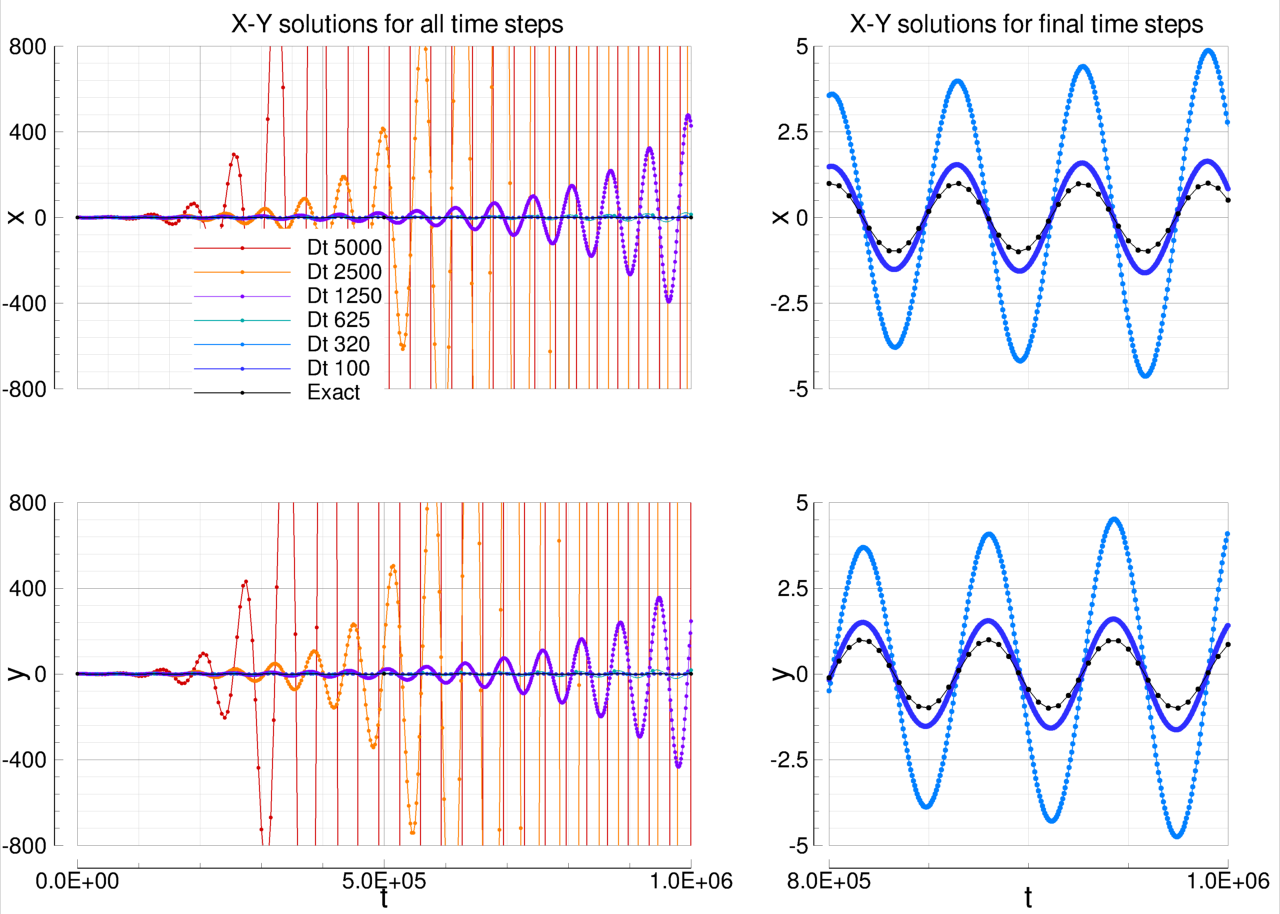
\includegraphics[width=1.00\textwidth]{errors-analysis/oscillation/errors_analysis-oscillation-adams-bashforth-1.png}
    \caption{1 step}\label{fig:results-oscillation-adams-bashforth-1}
  \end{subfigure}\quad%
  \begin{subfigure}[b]{0.45\textwidth}
    \centering
    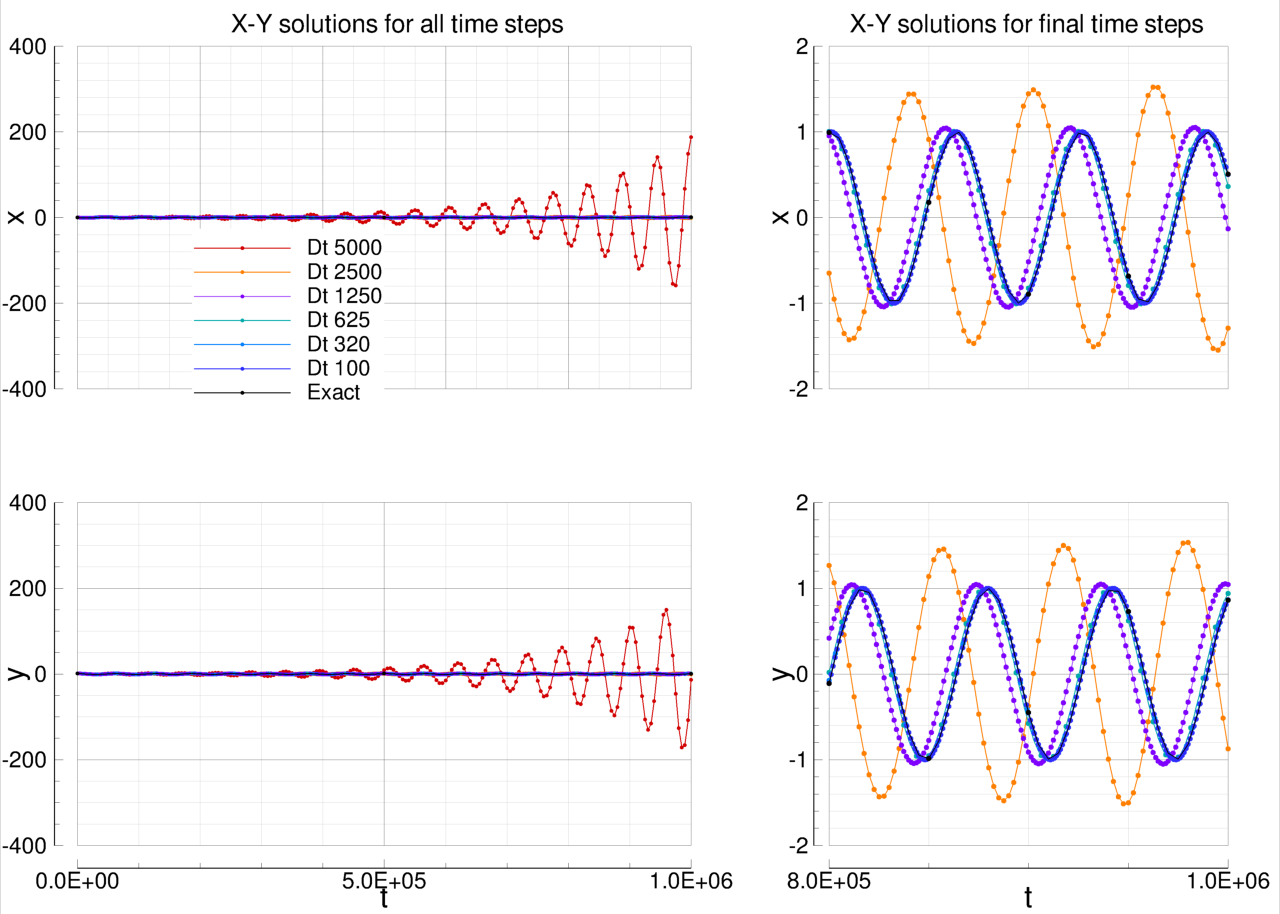
\includegraphics[width=1.00\textwidth]{errors-analysis/oscillation/errors_analysis-oscillation-adams-bashforth-2.png}
    \caption{2 steps}\label{fig:results-oscillation-adams-bashforth-2}
  \end{subfigure}\\
  \begin{subfigure}[b]{0.45\textwidth}
    \centering
    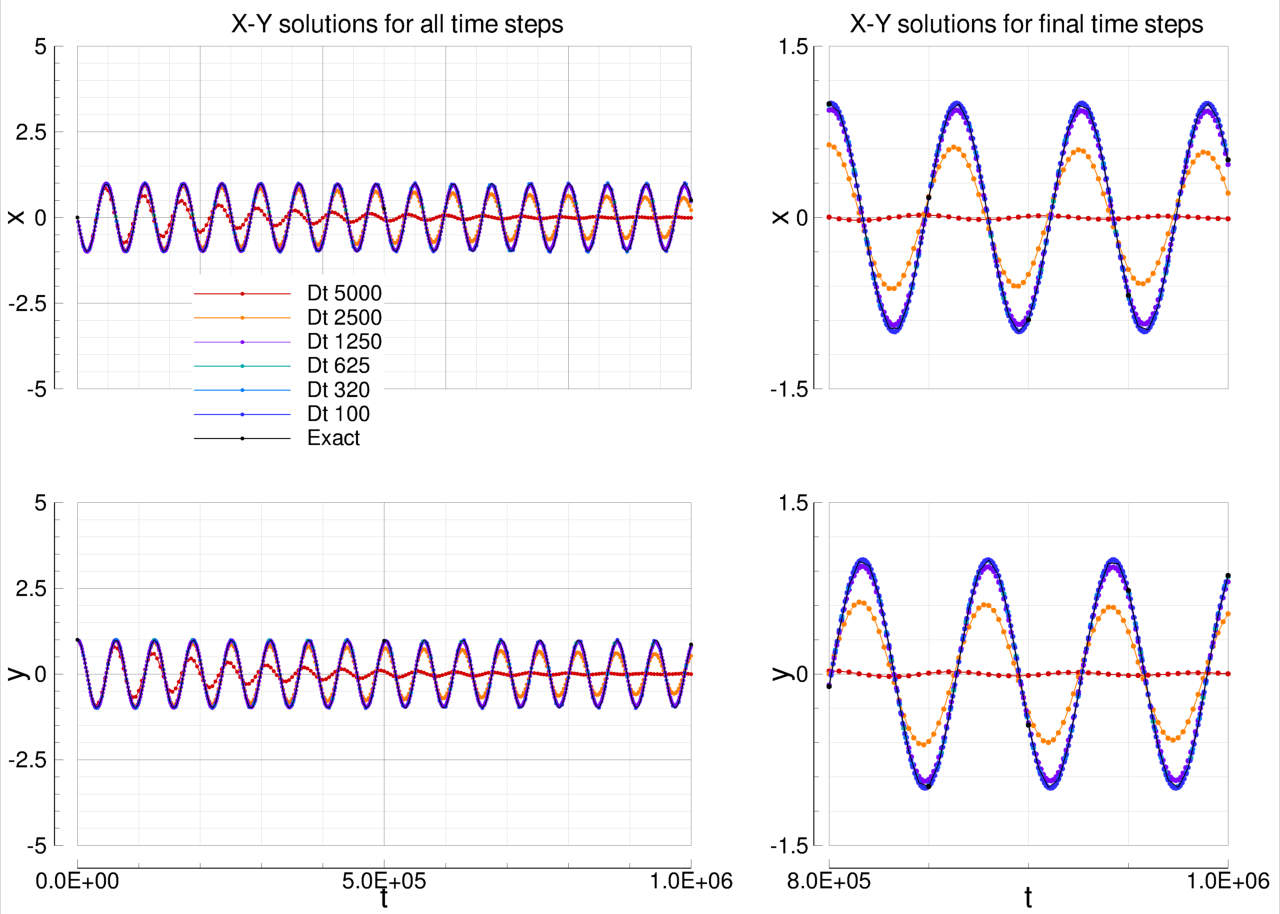
\includegraphics[width=1.00\textwidth]{errors-analysis/oscillation/errors_analysis-oscillation-adams-bashforth-3.png}
    \caption{3 steps}\label{fig:results-oscillation-adams-bashforth-3}
  \end{subfigure}\quad%
  \begin{subfigure}[b]{0.45\textwidth}
    \centering
    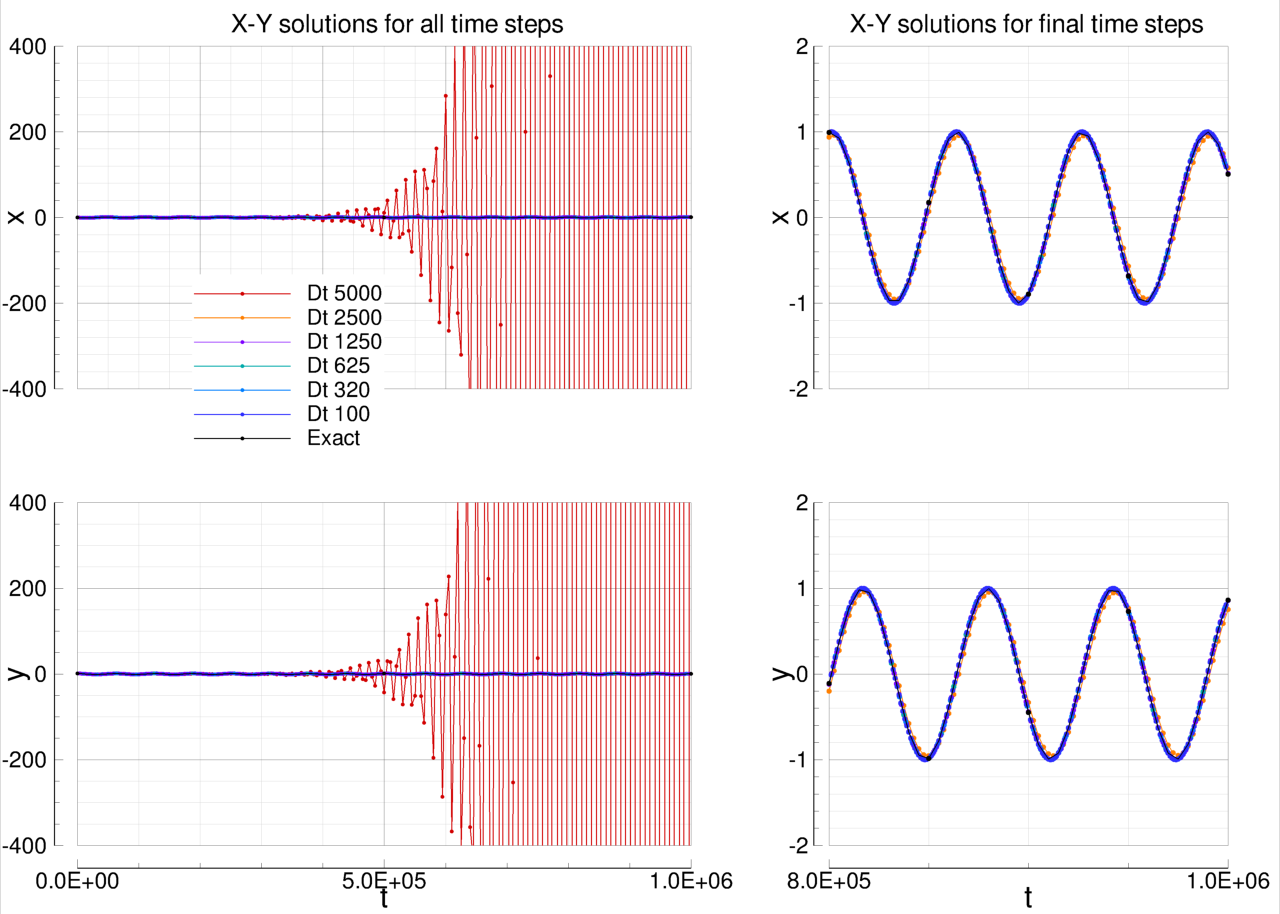
\includegraphics[width=1.00\textwidth]{errors-analysis/oscillation/errors_analysis-oscillation-adams-bashforth-4.png}
    \caption{4 steps}\label{fig:results-oscillation-adams-bashforth-4}
  \end{subfigure}
  \caption{Oscillation equations solutions computed by means of Adams-Bashforth solvers}\label{fig:results-oscillation-adams-bashforth}
\end{figure}



\subsubsection{Adams-Bashforth-Moulton}

Table \ref{tab:oscillation_errors_abm} summarizes the Adams-Bashforth-Moulton error analysis. The same considerations done for the Adams-Bashforth solutions can repeated for the Adams-Bashforth-Moulton ones, thus they are omitted for the sake of conciseness. An interesting result concerns the observed errors: the $O(10^{-2})$ error is now obtained with $\Delta t=1250$ for the 4-steps solver, thus it is 2 times faster than the corresponding Adams-Bashforth 4-step solver. Considering that the computational costs of a single Adams-Bashforth-Moulton step is only slightly greater than the corresponding Adamas-Bashforth step, the efficiency increasing is not negligible.

\begin{table}[!ht]
  \centering
  \caption{Oscillation test: errors analysis of predictor-corrector Adams-Bashforth-Moulton solvers}\label{tab:oscillation_errors_abm}
  \begin{subtable}[b]{0.40\textwidth}
    \centering
    \caption{1 step}\label{tab:oscillation-abm-1}
    \resizebox{1.00\textwidth}{!}{%
    \begin{tabular}{ccccc}
      \toprule
      {\sc Time Step} & {\sc Error X} & {\sc Error Y} & {\sc Order X} & {\sc Order Y} \\
      \hline
      5000.0          &  0.241E+20    &  0.266E+20    & /             & /             \\
      2500.0          &  0.664E+11    &  0.716E+11    & 28.44         & 28.47         \\
      1250.0          &  0.952E+06    &  0.100E+07    & 16.09         & 16.12         \\
       625.0          &  0.413E+04    &  0.407E+04    &  7.85         &  7.95         \\
       320.0          &  0.387E+03    &  0.383E+03    &  3.54         &  3.53         \\
       100.0          &  0.145E+03    &  0.145E+03    &  0.84         &  0.83         \\
      \bottomrule
    \end{tabular}}
  \end{subtable}\quad%
  \begin{subtable}[b]{0.40\textwidth}
    \centering
    \caption{2 steps}\label{tab:oscillation-abm-2}
    \resizebox{1.00\textwidth}{!}{%
    \begin{tabular}{ccccc}
      \toprule
      {\sc Time Step} & {\sc Error X} & {\sc Error Y} & {\sc Order X} & {\sc Order Y} \\
      \hline
      5000.0          &  0.704E+01    &  0.701E+01    & /             & /             \\
      2500.0          &  0.392E+01    &  0.395E+01    & 0.84          & 0.83          \\
      1250.0          &  0.148E+01    &  0.150E+01    & 1.40          & 1.39          \\
       625.0          &  0.526E+00    &  0.534E+00    & 1.49          & 1.49          \\
       320.0          &  0.193E+00    &  0.196E+00    & 1.50          & 1.50          \\
       100.0          &  0.338E-01    &  0.342E-01    & 1.50          & 1.50          \\
      \bottomrule
    \end{tabular}}
  \end{subtable}\\
  \begin{subtable}[b]{0.40\textwidth}
    \centering
    \caption{3 steps}\label{tab:oscillation-abm-3}
    \resizebox{1.00\textwidth}{!}{%
    \begin{tabular}{ccccc}
      \toprule
      {\sc Time Step} & {\sc Error X} & {\sc Error Y} & {\sc Order X} & {\sc Order Y} \\
      \hline
      5000.0          &  0.457E+01    &  0.464E+01    & /             & /             \\
      2500.0          &  0.656E+00    &  0.654E+00    & 2.80          & 2.83          \\
      1250.0          &  0.100E+00    &  0.987E-01    & 2.71          & 2.73          \\
       625.0          &  0.169E-01    &  0.167E-01    & 2.56          & 2.56          \\
       320.0          &  0.314E-02    &  0.310E-02    & 2.52          & 2.51          \\
       100.0          &  0.171E-03    &  0.169E-03    & 2.50          & 2.50          \\
      \bottomrule
    \end{tabular}}
  \end{subtable}\quad%
  \begin{subtable}[b]{0.40\textwidth}
    \centering
    \caption{4 steps}\label{tab:oscillation-abm-4}
    \resizebox{1.00\textwidth}{!}{%
    \begin{tabular}{ccccc}
      \toprule
      {\sc Time Step} & {\sc Error X} & {\sc Error Y} & {\sc Order X} & {\sc Order Y} \\
      \hline
      5000.0          &  0.229E+01    &  0.225E+01    & /             & /             \\
      2500.0          &  0.119E+00    &  0.118E+00    & 4.26          & 4.25          \\
      1250.0          &  0.825E-02    &  0.833E-02    & 3.85          & 3.83          \\
       625.0          &  0.671E-03    &  0.681E-03    & 3.62          & 3.61          \\
       320.0          &  0.631E-04    &  0.640E-04    & 3.53          & 3.53          \\
       100.0          &  0.107E-05    &  0.108E-05    & 3.51          & 3.51          \\
      \bottomrule
    \end{tabular}}
  \end{subtable}\\
\end{table}

Figure \ref{fig:results-oscillation-adams-bashforth-moulton} shows similar plots of figure \ref{fig:results-oscillation-adams-bashforth} above discussed. Differently from the Adams-Bashforth class, the amplitude damping feature is now possessed by the 2-steps solver, see plot \ref{fig:results-oscillation-adams-bashforth-moulton-2}, while all solutions show phase errors that decrease as the time resolution increases.

\begin{figure}[!ht]
  \centering
  \begin{subfigure}[b]{0.45\textwidth}
    \centering
    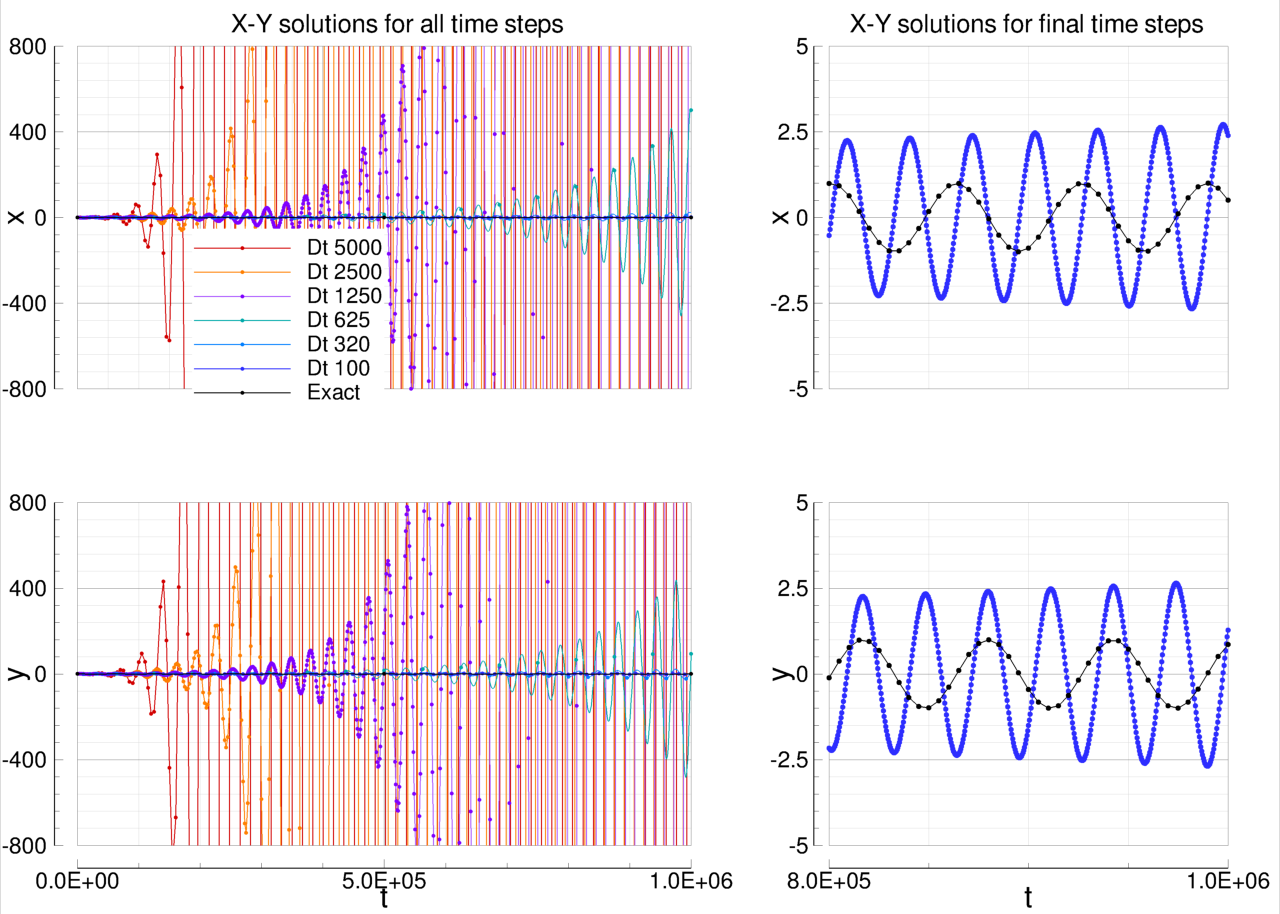
\includegraphics[width=1.00\textwidth]{errors-analysis/oscillation/errors_analysis-oscillation-adams-bashforth-moulton-1.png}
    \caption{1 step}\label{fig:results-oscillation-adams-bashforth-moulton-1}
  \end{subfigure}\quad%
  \begin{subfigure}[b]{0.45\textwidth}
    \centering
    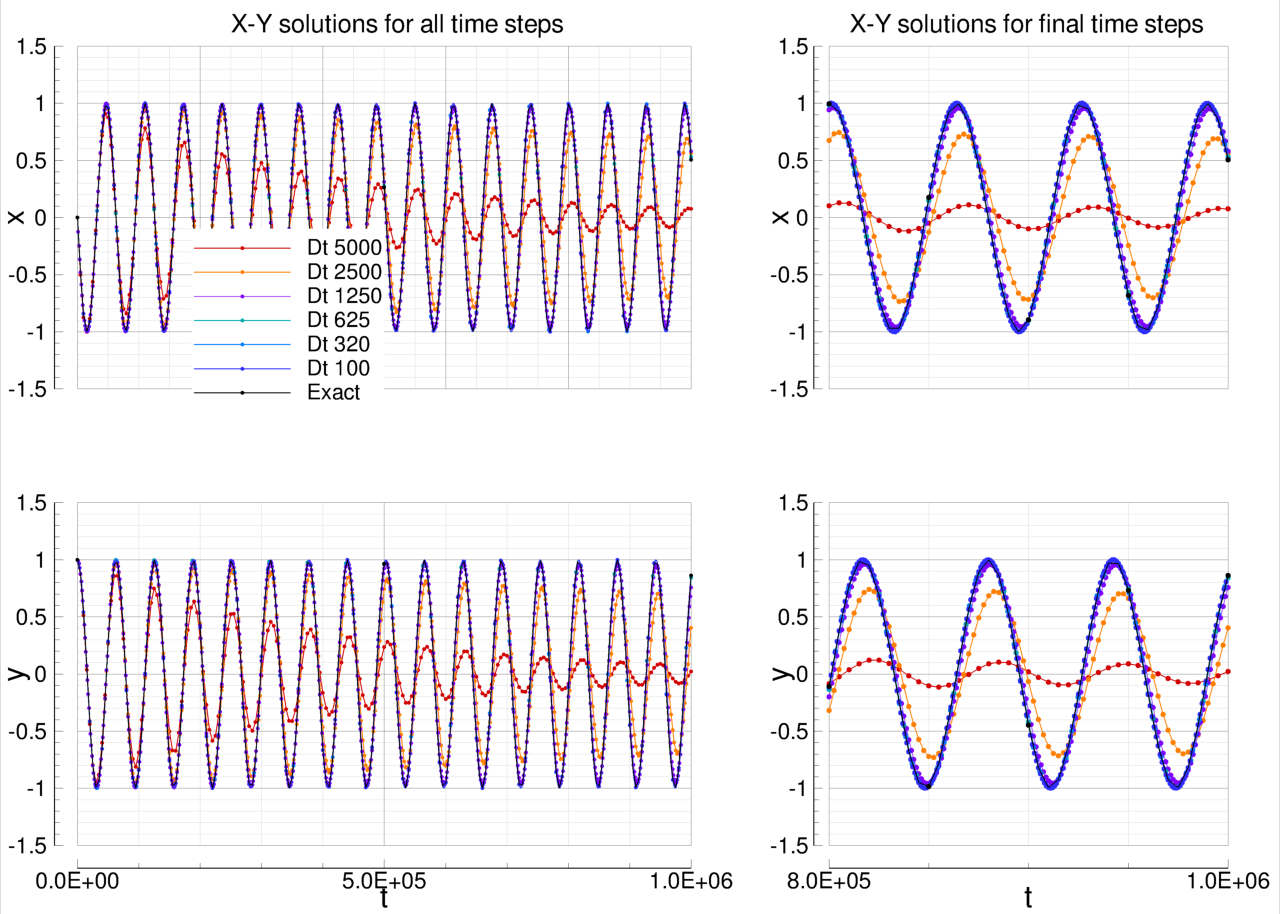
\includegraphics[width=1.00\textwidth]{errors-analysis/oscillation/errors_analysis-oscillation-adams-bashforth-moulton-2.png}
    \caption{2 steps}\label{fig:results-oscillation-adams-bashforth-moulton-2}
  \end{subfigure}\\
  \begin{subfigure}[b]{0.45\textwidth}
    \centering
    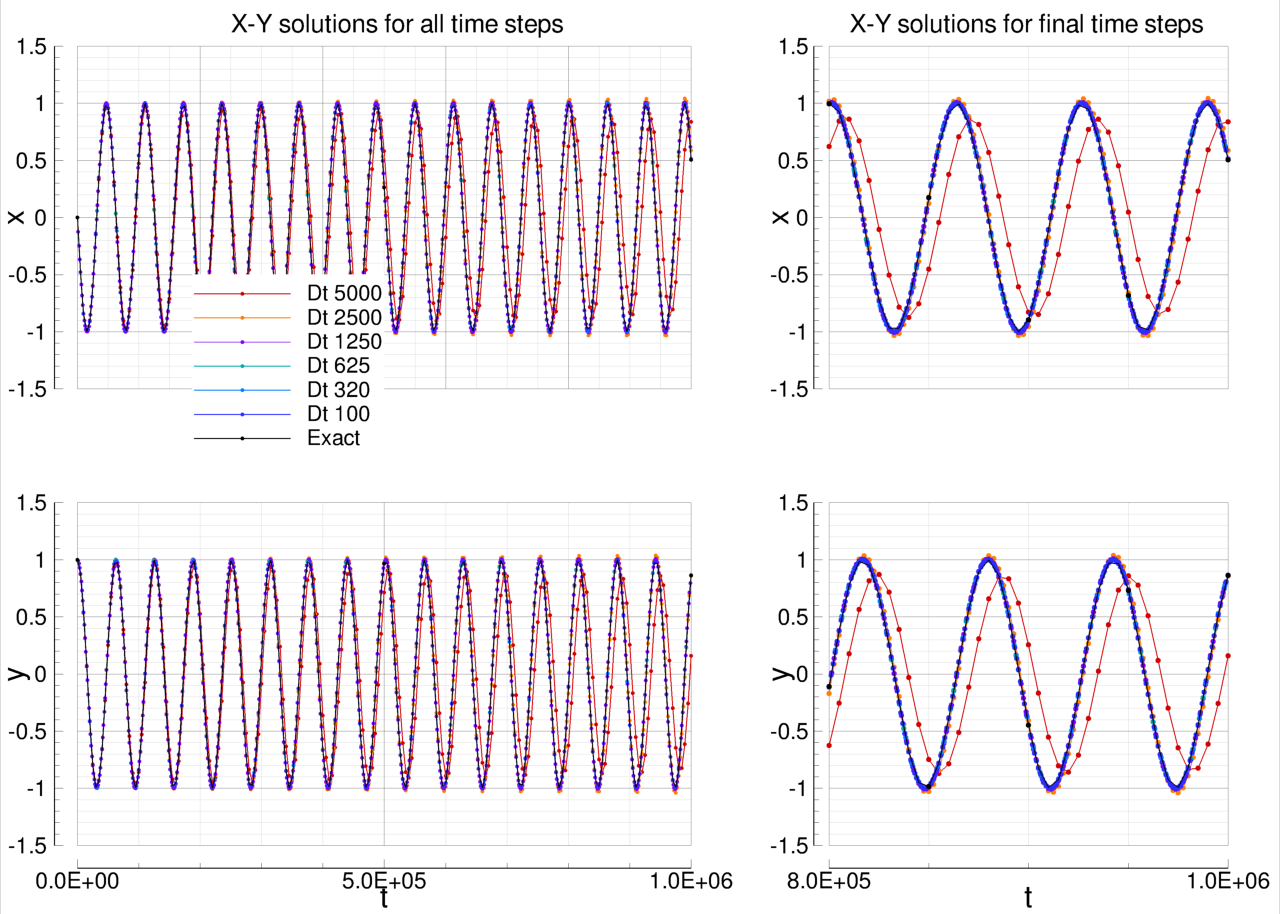
\includegraphics[width=1.00\textwidth]{errors-analysis/oscillation/errors_analysis-oscillation-adams-bashforth-moulton-3.png}
    \caption{3 steps}\label{fig:results-oscillation-adams-bashforth-moulton-3}
  \end{subfigure}\quad%
  \begin{subfigure}[b]{0.45\textwidth}
    \centering
    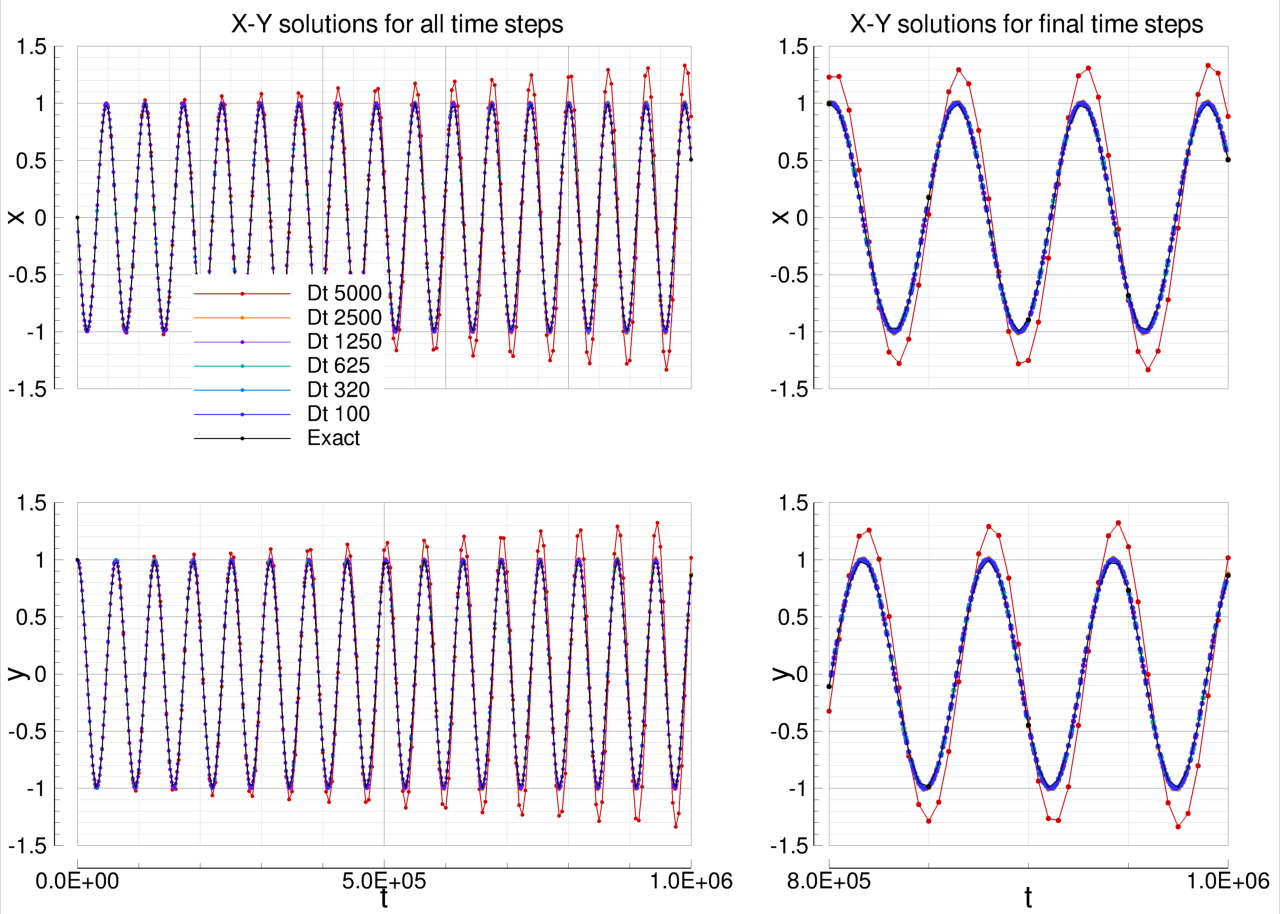
\includegraphics[width=1.00\textwidth]{errors-analysis/oscillation/errors_analysis-oscillation-adams-bashforth-moulton-4.png}
    \caption{4 steps}\label{fig:results-oscillation-adams-bashforth-moulton-4}
  \end{subfigure}
  \caption{Oscillation equations solutions computed by means of Adams-Bashforth-Moulton solvers}\label{fig:results-oscillation-adams-bashforth-moulton}
\end{figure}
\clearpage



\subsubsection{Adams-Moulton}

Table \ref{tab:oscillation_errors_am} summarizes the Adams-Moulton error analysis. The implicit Adams-Moulton solvers behave much like the Adams-Bashforth-Moulton ones: they have similar errors and observed orders for the same formal order considered. However, the implicit Adams-Moulton class uses one less step with respect the corresponding Adams-Bashforth-Moulton class: this could lead to the promise of higher computational efficiency. Notwithstanding, for solving the implicit non-linearity embedded into the Adams-Moulton solvers an iterative algorithm must be employed: for the results presented, a 5 iterations of \emph{fixed point algorithm} have been computed. This strongly reduces the eventual gain of computational efficiency with respect the Adams-Bashforth-Moulton class.

\begin{table}[!ht]
  \centering
  \caption{Oscillation test: errors analysis of explicit Adams-Moulton solvers; the implicit non-linearity is solved by 5 iterations of \emph{fixed point algorithm}}\label{tab:oscillation_errors_am}
  \begin{subtable}[b]{0.40\textwidth}
    \centering
    \caption{1 step}\label{tab:oscillation-am-1}
    \resizebox{1.00\textwidth}{!}{%
    \begin{tabular}{ccccc}
      \toprule
      {\sc Time Step} & {\sc Error X} & {\sc Error Y} & {\sc Order X} & {\sc Order Y} \\
      \hline
      5000.0          &  0.840E+10    &  0.706E+10    & /             & /             \\
      2500.0          &  0.503E+06    &  0.570E+06    & 14.03         & 13.60         \\
      1250.0          &  0.289E+04    &  0.272E+04    &  7.45         &  7.71         \\
       625.0          &  0.239E+03    &  0.232E+03    &  3.59         &  3.55         \\
       320.0          &  0.737E+02    &  0.722E+02    &  1.76         &  1.74         \\
       100.0          &  0.250E+02    &  0.247E+02    &  0.93         &  0.92         \\
      \bottomrule
    \end{tabular}}
  \end{subtable}\quad%
  \begin{subtable}[b]{0.40\textwidth}
    \centering
    \caption{2 steps}\label{tab:oscillation-am-2}
    \resizebox{1.00\textwidth}{!}{%
    \begin{tabular}{ccccc}
      \toprule
      {\sc Time Step} & {\sc Error X} & {\sc Error Y} & {\sc Order X} & {\sc Order Y} \\
      \hline
      5000.0          &  0.108E+02    &  0.109E+02    & /             & /             \\
      2500.0          &  0.412E+01    &  0.419E+01    & 1.39          & 1.38          \\
      1250.0          &  0.148E+01    &  0.150E+01    & 1.48          & 1.48          \\
       625.0          &  0.527E+00    &  0.533E+00    & 1.49          & 1.49          \\
       320.0          &  0.193E+00    &  0.196E+00    & 1.50          & 1.50          \\
       100.0          &  0.338E-01    &  0.342E-01    & 1.50          & 1.50          \\
      \bottomrule
    \end{tabular}}
  \end{subtable}\\
  \begin{subtable}[b]{0.40\textwidth}
    \centering
    \caption{3 steps}\label{tab:oscillation-am-3}
    \resizebox{1.00\textwidth}{!}{%
    \begin{tabular}{ccccc}
      \toprule
      {\sc Time Step} & {\sc Error X} & {\sc Error Y} & {\sc Order X} & {\sc Order Y} \\
      \hline
      5000.0          &  0.390E+01    &  0.384E+01    & /             & /             \\
      2500.0          &  0.551E+00    &  0.544E+00    & 2.82          & 2.82          \\
      1250.0          &  0.947E-01    &  0.934E-01    & 2.54          & 2.54          \\
       625.0          &  0.167E-01    &  0.165E-01    & 2.50          & 2.50          \\
       320.0          &  0.313E-02    &  0.309E-02    & 2.50          & 2.50          \\
       100.0          &  0.171E-03    &  0.169E-03    & 2.50          & 2.50          \\
      \bottomrule
    \end{tabular}}
  \end{subtable}\quad%
  \begin{subtable}[b]{0.40\textwidth}
    \centering
    \caption{4 steps}\label{tab:oscillation-am-4}
    \resizebox{1.00\textwidth}{!}{%
    \begin{tabular}{ccccc}
      \toprule
      {\sc Time Step} & {\sc Error X} & {\sc Error Y} & {\sc Order X} & {\sc Order Y} \\
      \hline
      5000.0          &  0.983E+00    &  0.999E+00    & /             & /             \\
      2500.0          &  0.832E-01    &  0.845E-01    & 3.56          & 3.56          \\
      1250.0          &  0.736E-02    &  0.746E-02    & 3.50          & 3.50          \\
       625.0          &  0.652E-03    &  0.660E-03    & 3.50          & 3.50          \\
       320.0          &  0.626E-04    &  0.635E-04    & 3.50          & 3.50          \\
       100.0          &  0.107E-05    &  0.108E-05    & 3.50          & 3.50          \\
      \bottomrule
    \end{tabular}}
  \end{subtable}\\
\end{table}

Figure \ref{fig:results-oscillation-adams-moulton} shows similar plots of figure \ref{fig:results-oscillation-adams-bashforth-moulton} above discussed: there are not relevant differences between the 2 classes of solvers.

\begin{figure}[!ht]
  \centering
  \begin{subfigure}[b]{0.45\textwidth}
    \centering
    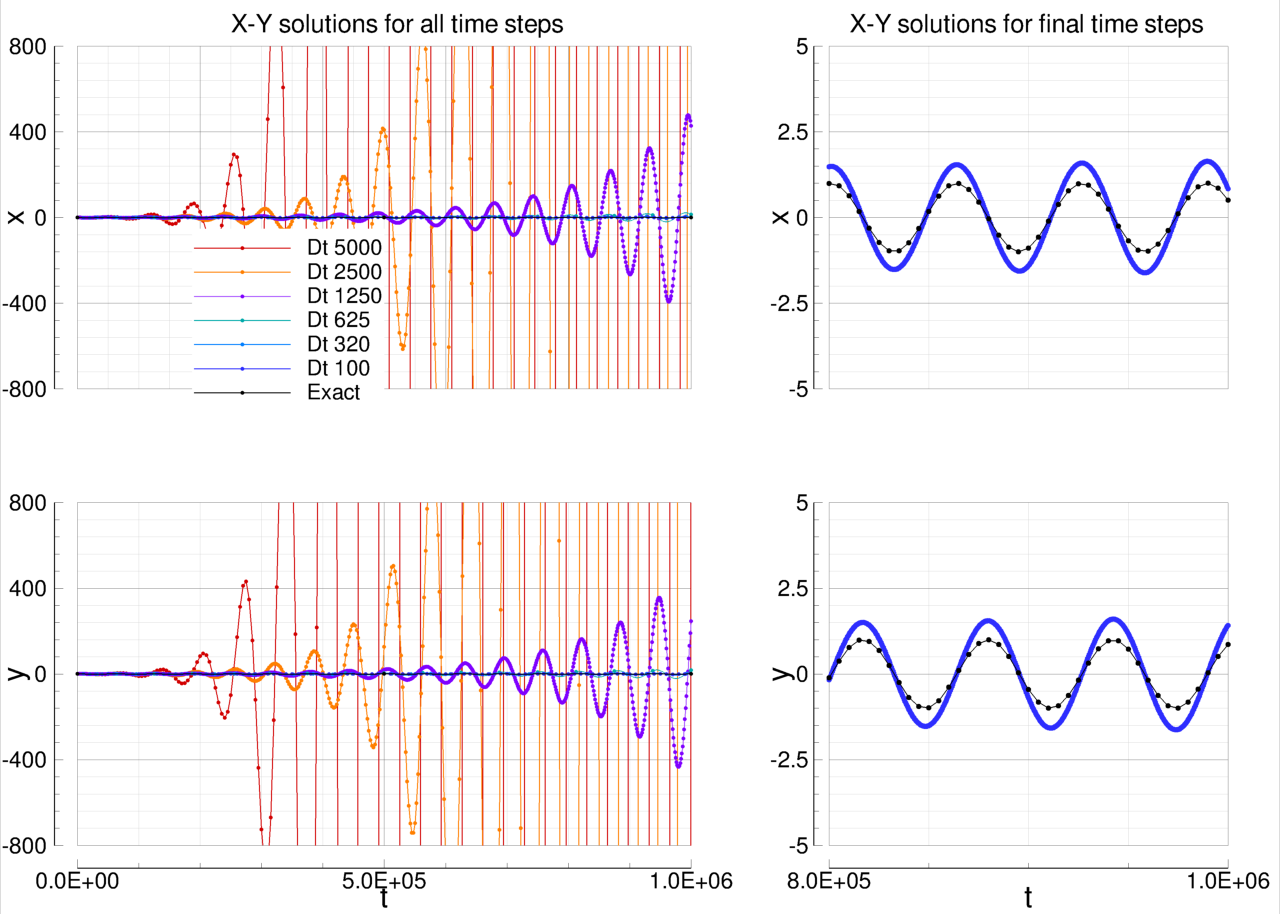
\includegraphics[width=1.00\textwidth]{errors-analysis/oscillation/errors_analysis-oscillation-adams-moulton-0.png}
    \caption{0 step}\label{fig:results-oscillation-adams-moulton-0}
  \end{subfigure}\quad%
  \begin{subfigure}[b]{0.45\textwidth}
    \centering
    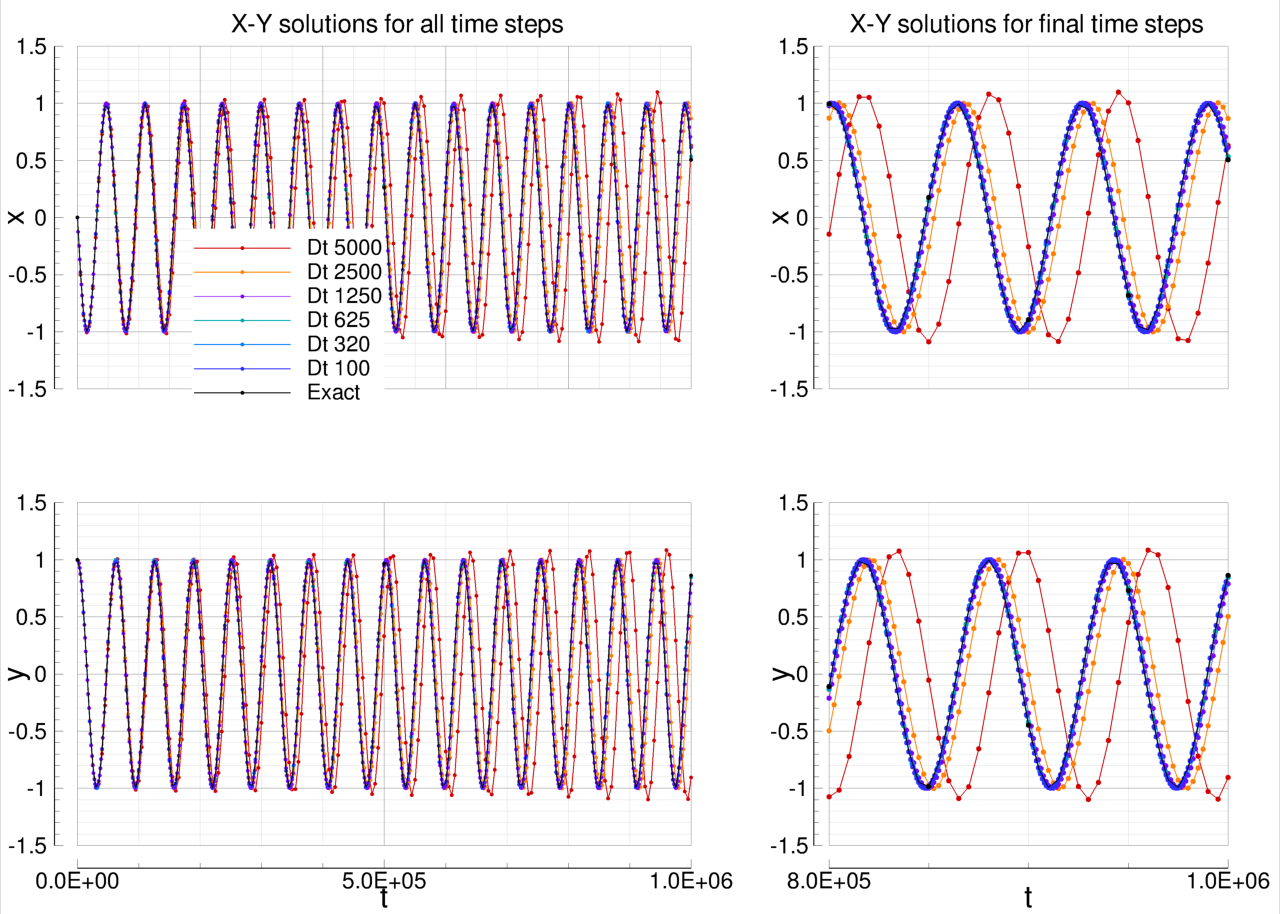
\includegraphics[width=1.00\textwidth]{errors-analysis/oscillation/errors_analysis-oscillation-adams-moulton-1.png}
    \caption{1 step}\label{fig:results-oscillation-adams-moulton-1}
  \end{subfigure}\\
  \begin{subfigure}[b]{0.45\textwidth}
    \centering
    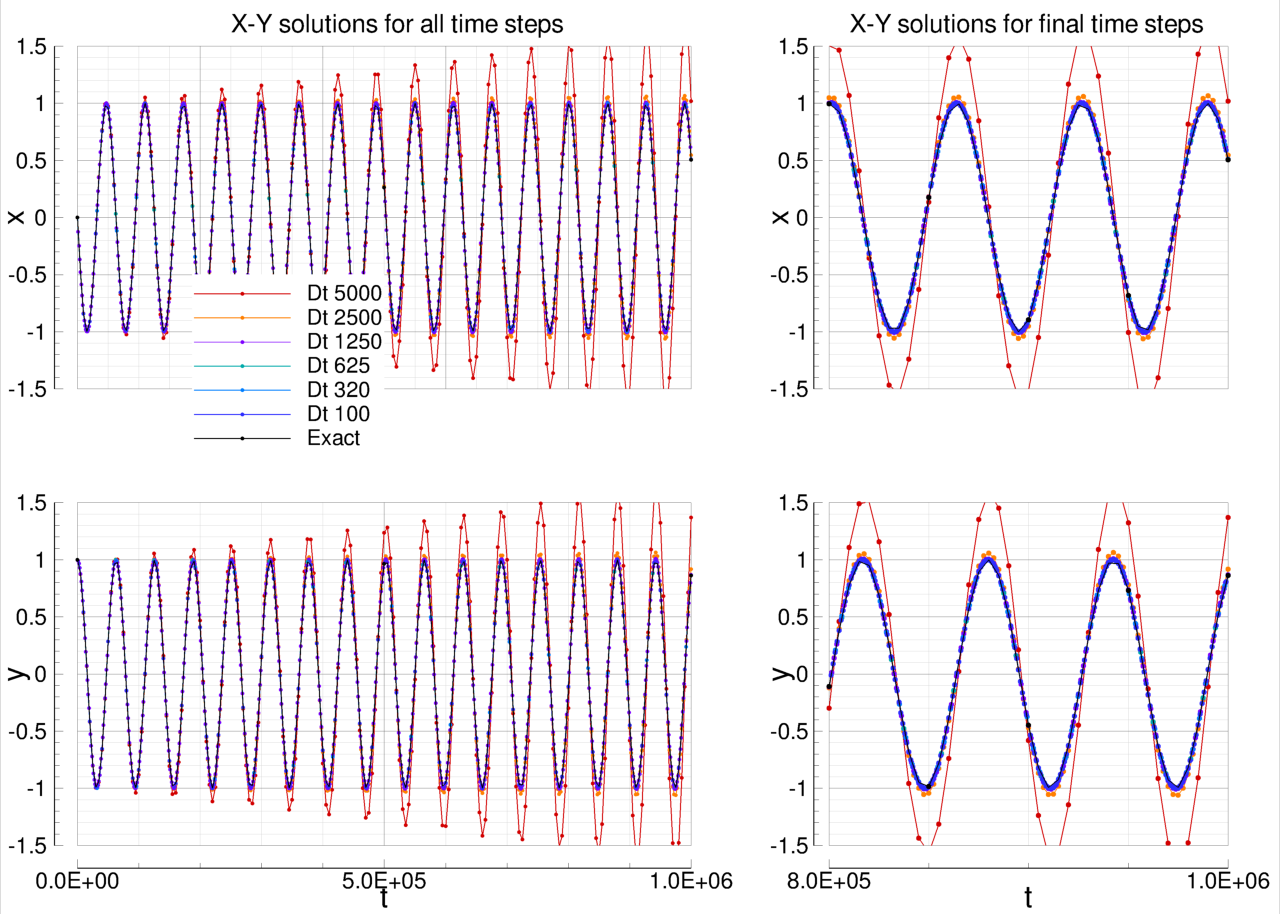
\includegraphics[width=1.00\textwidth]{errors-analysis/oscillation/errors_analysis-oscillation-adams-moulton-2.png}
    \caption{2 steps}\label{fig:results-oscillation-adams-moulton-2}
  \end{subfigure}\quad%
  \begin{subfigure}[b]{0.45\textwidth}
    \centering
    \includegraphics[width=1.00\textwidth]{errors-analysis/oscillation/errors_analysis-oscillation-adams-moulton-3.png}
    \caption{3 steps}\label{fig:results-oscillation-adams-moulton-3}
  \end{subfigure}
  \caption{Oscillation equations solutions computed by means of Adams-Moulton solvers}\label{fig:results-oscillation-adams-moulton}
\end{figure}



\subsubsection{Leapfrog}

The Leapfrog solutions are in agreement with the expected results: both unfiltered and RAW-filtered solutions show an observed order of accuracy that tends to the formal $2^{nd}$ order. The two solutions are almost the same.

\begin{table}[!ht]
  \centering
  \caption{Oscillation test: errors analysis of explicit Leapfrog solvers}\label{tab:oscillation_errors_lf}
  \begin{subtable}[b]{0.40\textwidth}
    \centering
    \caption{Unfiltered}\label{tab:oscillation-leapfrog}
    \resizebox{1.00\textwidth}{!}{%
    \begin{tabular}{ccccc}
      \toprule
      {\sc Time Step} & {\sc Error X} & {\sc Error Y} & {\sc Order X} & {\sc Order Y} \\
      \hline
      5000.0          &  0.156E+02    &  0.156E+02    & /             & /             \\
      2500.0          &  0.849E+01    &  0.846E+01    & 0.87          & 0.88          \\
      1250.0          &  0.300E+01    &  0.303E+01    & 1.50          & 1.48          \\
       625.0          &  0.106E+01    &  0.107E+01    & 1.51          & 1.50          \\
       320.0          &  0.387E+00    &  0.392E+00    & 1.50          & 1.50          \\
       100.0          &  0.676E-01    &  0.685E-01    & 1.50          & 1.50          \\
      \bottomrule
    \end{tabular}}
  \end{subtable}\quad%
  \begin{subtable}[b]{0.40\textwidth}
    \centering
    \caption{RAW-filtered}\label{tab:oscillation-leapfrog-raw}
    \resizebox{1.00\textwidth}{!}{%
    \begin{tabular}{ccccc}
      \toprule
      {\sc Time Step} & {\sc Error X} & {\sc Error Y} & {\sc Order X} & {\sc Order Y} \\
      \hline
      5000.0          &  0.156E+02    &  0.156E+02    & /             & /             \\
      2500.0          &  0.855E+01    &  0.852E+01    & 0.86          & 0.87          \\
      1250.0          &  0.303E+01    &  0.305E+01    & 1.50          & 1.48          \\
       625.0          &  0.107E+01    &  0.108E+01    & 1.51          & 1.50          \\
       320.0          &  0.390E+00    &  0.395E+00    & 1.50          & 1.50          \\
       100.0          &  0.685E-01    &  0.692E-01    & 1.50          & 1.50          \\
      \bottomrule
    \end{tabular}}
  \end{subtable}\\
\end{table}

\begin{figure}[!ht]
  \centering
  \begin{subfigure}[b]{0.45\textwidth}
    \centering
    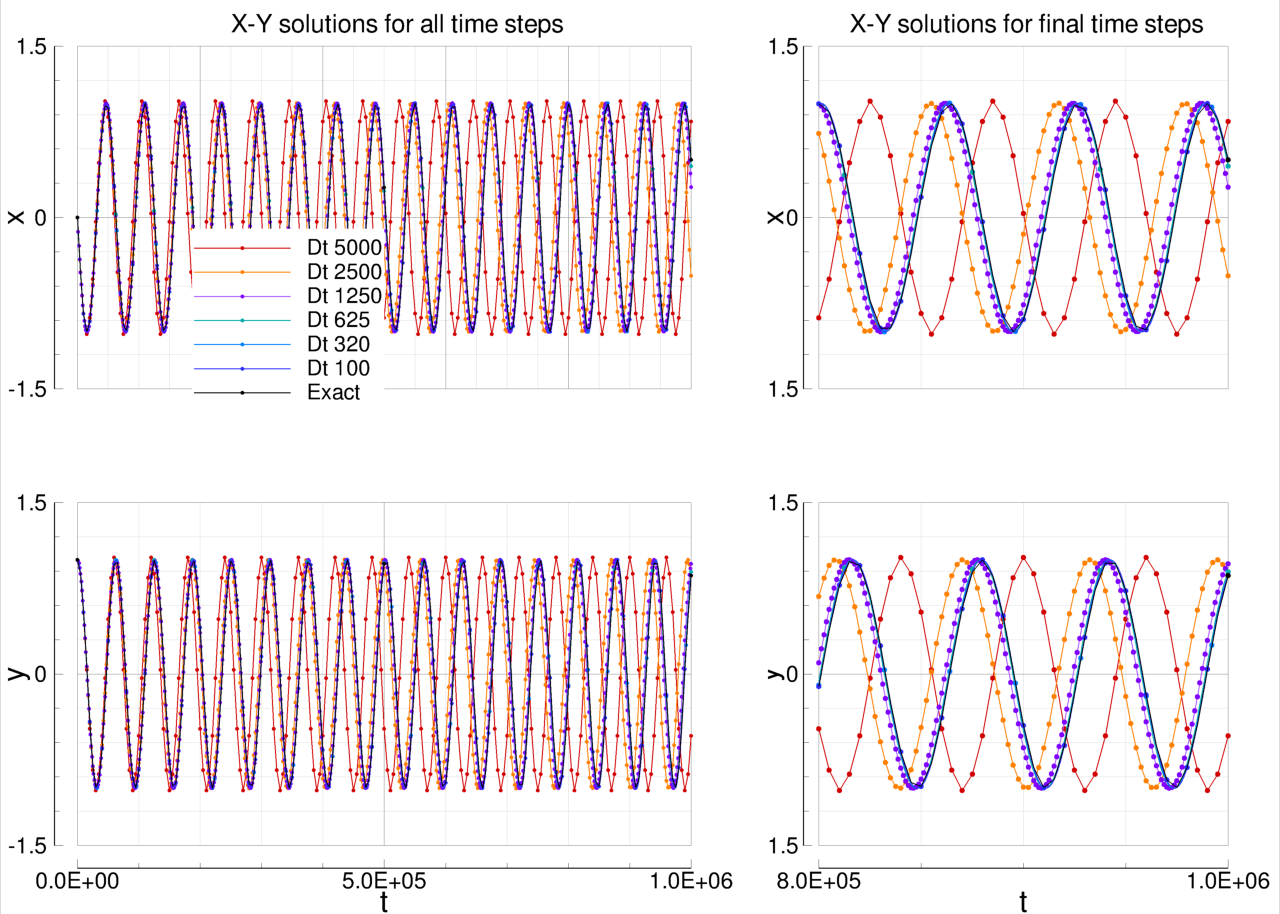
\includegraphics[width=1.00\textwidth]{errors-analysis/oscillation/errors_analysis-oscillation-leapfrog.png}
    \caption{Unfiltered}\label{fig:results-oscillation-leapfrog-unfiltered}
  \end{subfigure}\quad%
  \begin{subfigure}[b]{0.45\textwidth}
    \centering
    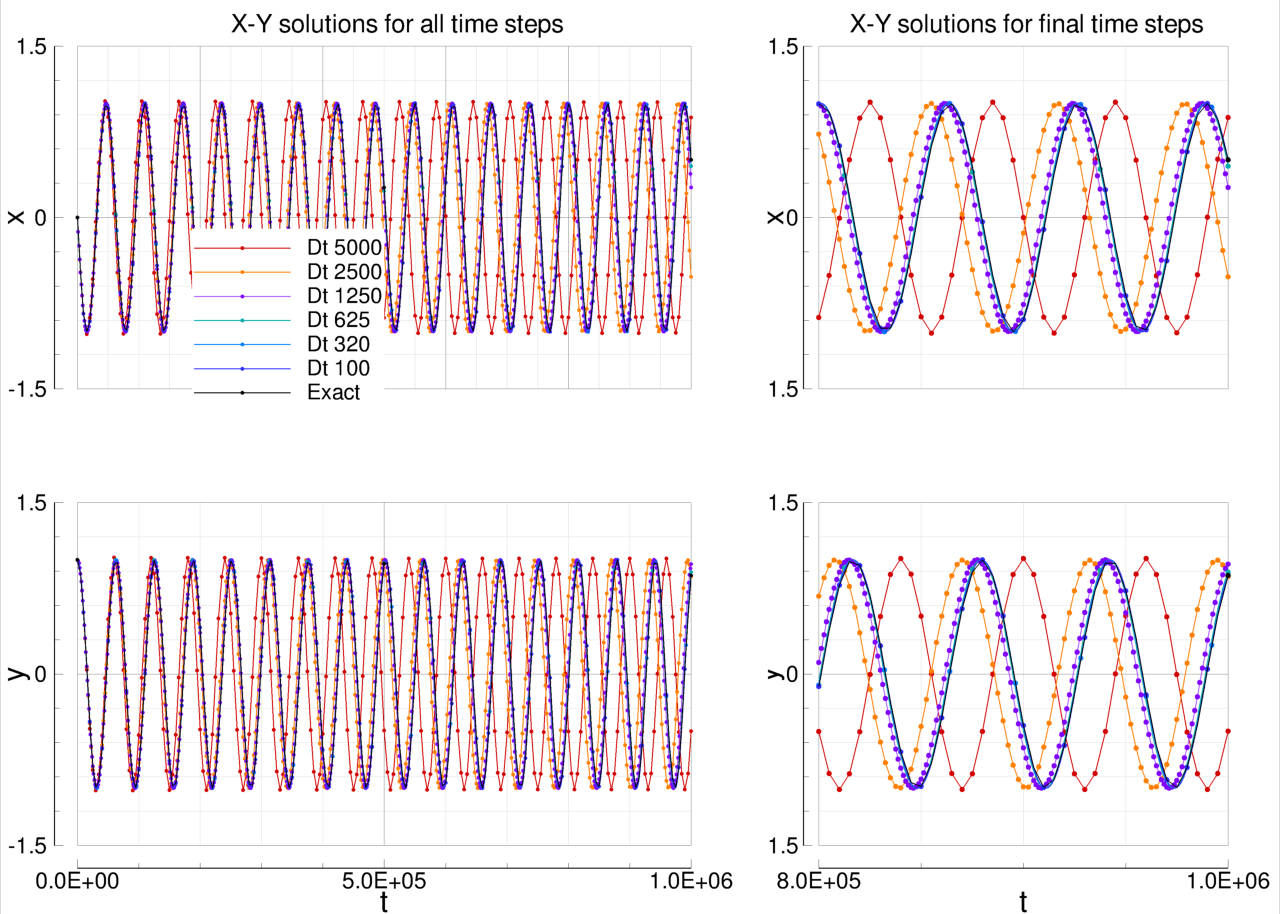
\includegraphics[width=1.00\textwidth]{errors-analysis/oscillation/errors_analysis-oscillation-leapfrog-raw.png}
    \caption{RAW-filtered}\label{fig:results-oscillation-leapfrog-raw}
  \end{subfigure}
  \caption{Oscillation equations solutions computed by means of Leapfrog solvers}\label{fig:results-oscillation-leapfrog}
\end{figure}



\subsubsection{Low Storage Runge-Kutta}

\begin{table}[!ht]
  \centering
  \caption{Oscillation test: errors analysis of explicit Low Storage Runge-Kutta solvers}\label{tab:oscillation_errors_ls_rk}
  \begin{subtable}[b]{0.40\textwidth}
    \centering
    \caption{1 stage}\label{tab:oscillation-ls-rk-1}
    \resizebox{1.00\textwidth}{!}{%
    \begin{tabular}{ccccc}
      \toprule
      {\sc Time Step} & {\sc Error X} & {\sc Error Y} & {\sc Order X} & {\sc Order Y} \\
      \hline
      5000.0          &  0.840E+10    &  0.706E+10    & /             & /             \\
      2500.0          &  0.503E+06    &  0.570E+06    & 14.03         & 13.60         \\
      1250.0          &  0.289E+04    &  0.272E+04    &  7.45         &  7.71         \\
       625.0          &  0.239E+03    &  0.232E+03    &  3.59         &  3.55         \\
       320.0          &  0.737E+02    &  0.722E+02    &  1.76         &  1.74         \\
       100.0          &  0.250E+02    &  0.247E+02    &  0.93         &  0.92         \\
      \bottomrule
    \end{tabular}}
  \end{subtable}\quad%
  \begin{subtable}[b]{0.40\textwidth}
    \centering
    \caption{5 stages}\label{tab:oscillation-ls-rk-5}
    \resizebox{1.00\textwidth}{!}{%
    \begin{tabular}{ccccc}
      \toprule
      {\sc Time Step} & {\sc Error X} & {\sc Error Y} & {\sc Order X} & {\sc Order Y} \\
      \hline
      5000.0          &  0.120E+00    &  0.122E+00    & /             & /             \\
      2500.0          &  0.106E-01    &  0.107E-01    & 3.51          & 3.51          \\
      1250.0          &  0.935E-03    &  0.947E-03    & 3.50          & 3.50          \\
       625.0          &  0.826E-04    &  0.836E-04    & 3.50          & 3.50          \\
       320.0          &  0.793E-05    &  0.803E-05    & 3.50          & 3.50          \\
       100.0          &  0.135E-06    &  0.137E-06    & 3.50          & 3.50          \\
      \bottomrule
    \end{tabular}}
  \end{subtable}\\
  \begin{subtable}[b]{0.40\textwidth}
    \centering
    \caption{6 stages}\label{tab:oscillation-ls-rk-6}
    \resizebox{1.00\textwidth}{!}{%
    \begin{tabular}{ccccc}
      \toprule
      {\sc Time Step} & {\sc Error X} & {\sc Error Y} & {\sc Order X} & {\sc Order Y} \\
      \hline
      5000.0          &  0.979E-01    &  0.994E-01    & /             & /             \\
      2500.0          &  0.876E-02    &  0.888E-02    & 3.48          & 3.48          \\
      1250.0          &  0.776E-03    &  0.786E-03    & 3.50          & 3.50          \\
       625.0          &  0.686E-04    &  0.695E-04    & 3.50          & 3.50          \\
       320.0          &  0.659E-05    &  0.667E-05    & 3.50          & 3.50          \\
       100.0          &  0.112E-06    &  0.114E-06    & 3.50          & 3.50          \\
      \bottomrule
    \end{tabular}}
  \end{subtable}\quad%
  \begin{subtable}[b]{0.40\textwidth}
    \centering
    \caption{7 stages}\label{tab:oscillation-ls-rk-7}
    \resizebox{1.00\textwidth}{!}{%
    \begin{tabular}{ccccc}
      \toprule
      {\sc Time Step} & {\sc Error X} & {\sc Error Y} & {\sc Order X} & {\sc Order Y} \\
      \hline
      5000.0          &  0.238E-01    &  0.240E-01    & /             & /             \\
      2500.0          &  0.203E-02    &  0.205E-02    & 3.55          & 3.55          \\
      1250.0          &  0.177E-03    &  0.180E-03    & 3.51          & 3.51          \\
       625.0          &  0.156E-04    &  0.158E-04    & 3.50          & 3.50          \\
       320.0          &  0.150E-05    &  0.152E-05    & 3.50          & 3.50          \\
       100.0          &  0.269E-07    &  0.273E-07    & 3.46          & 3.46          \\
      \bottomrule
    \end{tabular}}
  \end{subtable}\\
  \begin{subtable}[b]{0.40\textwidth}
    \centering
    \caption{12 stages}\label{tab:oscillation-ls-rk-12}
    \resizebox{1.00\textwidth}{!}{%
    \begin{tabular}{ccccc}
      \toprule
      {\sc Time Step} & {\sc Error X} & {\sc Error Y} & {\sc Order X} & {\sc Order Y} \\
      \hline
      5000.0          &  0.195E-01    &  0.198E-01    & /             & /             \\
      2500.0          &  0.175E-02    &  0.177E-02    & 3.48          & 3.48          \\
      1250.0          &  0.155E-03    &  0.157E-03    & 3.50          & 3.50          \\
       625.0          &  0.137E-04    &  0.139E-04    & 3.50          & 3.50          \\
       320.0          &  0.132E-05    &  0.133E-05    & 3.50          & 3.50          \\
       100.0          &  0.225E-07    &  0.228E-07    & 3.50          & 3.50          \\
      \bottomrule
    \end{tabular}}
  \end{subtable}\quad%
  \begin{subtable}[b]{0.40\textwidth}
    \centering
    \caption{13 stages}\label{tab:oscillation-ls-rk-13}
    \resizebox{1.00\textwidth}{!}{%
    \begin{tabular}{ccccc}
      \toprule
      {\sc Time Step} & {\sc Error X} & {\sc Error Y} & {\sc Order X} & {\sc Order Y} \\
      \hline
      5000.0          &  0.795E-02    &  0.805E-02    & /             & /             \\
      2500.0          &  0.703E-03    &  0.712E-03    & 3.50          & 3.50          \\
      1250.0          &  0.621E-04    &  0.629E-04    & 3.50          & 3.50          \\
       625.0          &  0.549E-05    &  0.556E-05    & 3.50          & 3.50          \\
       320.0          &  0.527E-06    &  0.534E-06    & 3.50          & 3.50          \\
       100.0          &  0.899E-08    &  0.911E-08    & 3.50          & 3.50          \\
      \bottomrule
    \end{tabular}}
  \end{subtable}\\
  \begin{subtable}[b]{0.40\textwidth}
    \centering
    \caption{14 stages}\label{tab:oscillation-ls-rk-14}
    \resizebox{1.00\textwidth}{!}{%
    \begin{tabular}{ccccc}
      \toprule
      {\sc Time Step} & {\sc Error X} & {\sc Error Y} & {\sc Order X} & {\sc Order Y} \\
      \hline
      5000.0          &  0.849E-02    &  0.860E-02    & /             & /             \\
      2500.0          &  0.750E-03    &  0.759E-03    & 3.50          & 3.50          \\
      1250.0          &  0.662E-04    &  0.671E-04    & 3.50          & 3.50          \\
       625.0          &  0.585E-05    &  0.593E-05    & 3.50          & 3.50          \\
       320.0          &  0.562E-06    &  0.569E-06    & 3.50          & 3.50          \\
       100.0          &  0.959E-08    &  0.972E-08    & 3.50          & 3.50          \\
      \bottomrule
    \end{tabular}}
  \end{subtable}\quad%
\end{table}

\begin{figure}[!ht]
  \centering
  \begin{subfigure}[b]{0.45\textwidth}
    \centering
    \includegraphics[width=1.00\textwidth]{errors-analysis/oscillation/errors_analysis-oscillation-ls-runge-kutta-1.png}
    \caption{1 stage}\label{fig:results-oscillation-ls-runge-kutta-1}
  \end{subfigure}\quad%
  \begin{subfigure}[b]{0.45\textwidth}
    \centering
    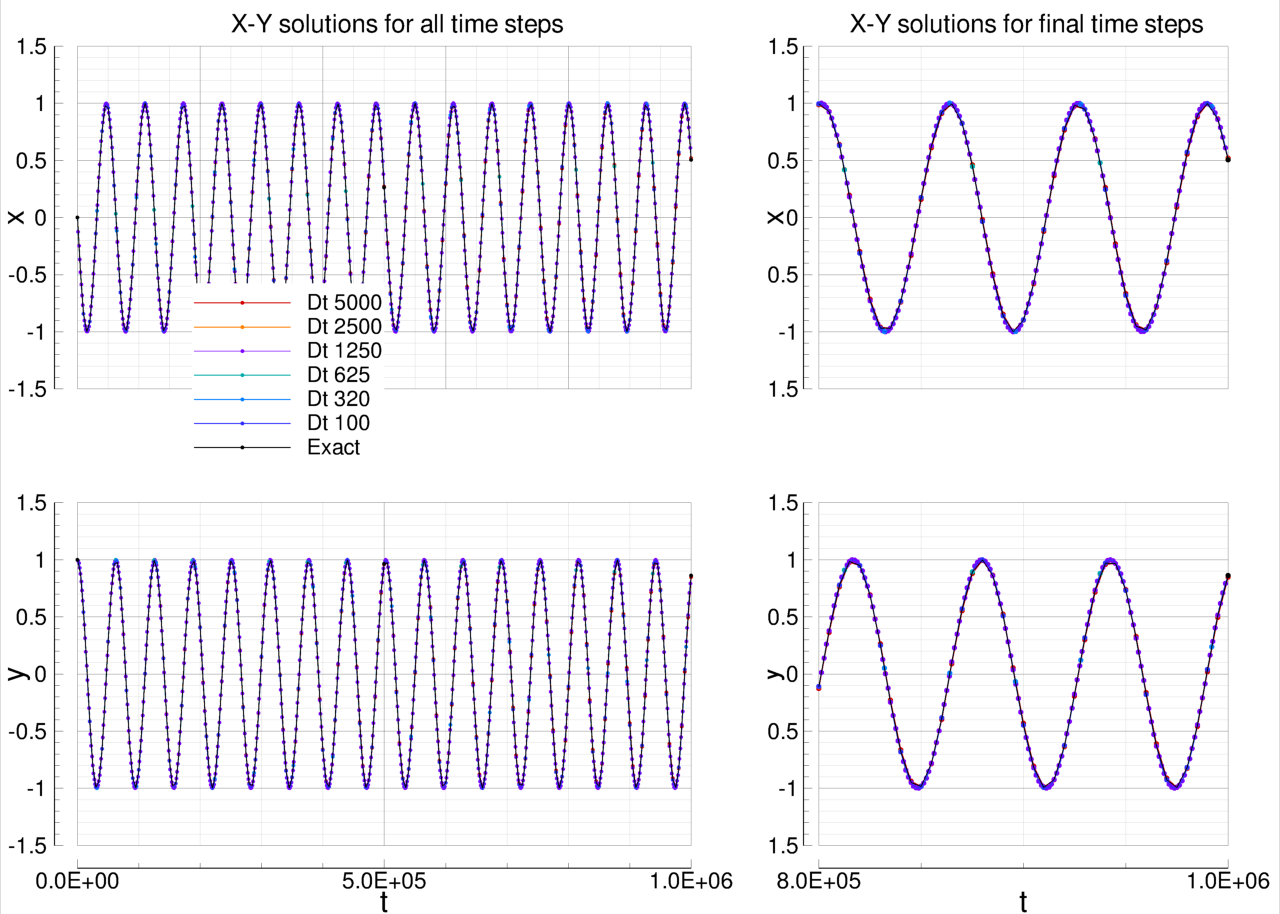
\includegraphics[width=1.00\textwidth]{errors-analysis/oscillation/errors_analysis-oscillation-ls-runge-kutta-5.png}
    \caption{5 stages}\label{fig:results-oscillation-ls-runge-kutta-5}
  \end{subfigure}
  \caption{Oscillation equations solutions computed by means of low storage Runge-Kutta solvers}\label{fig:results-oscillation-ls-runge-kutta-1-5}
\end{figure}

\begin{figure}[!ht]
  \centering
  \begin{subfigure}[b]{0.45\textwidth}
    \centering
    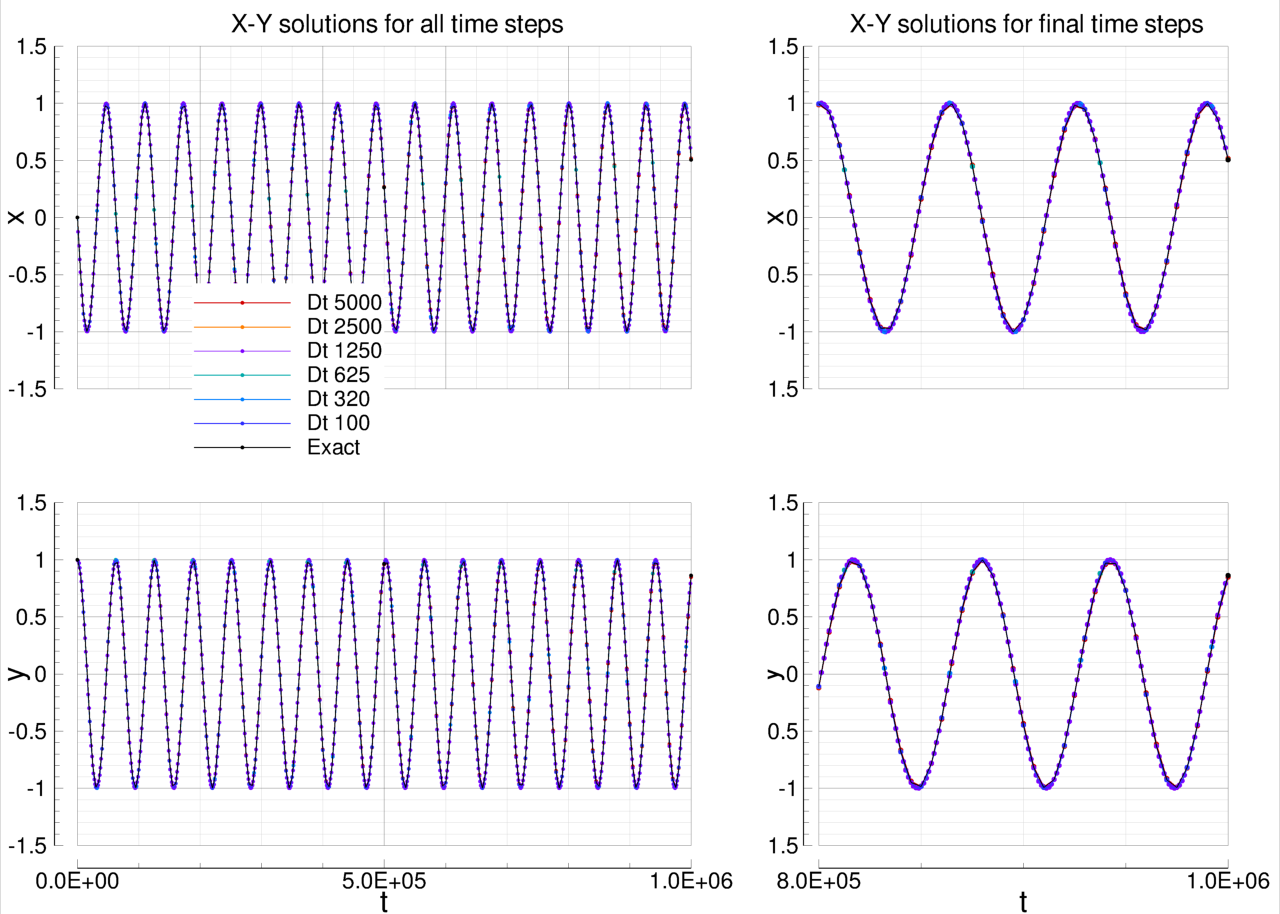
\includegraphics[width=1.00\textwidth]{errors-analysis/oscillation/errors_analysis-oscillation-ls-runge-kutta-6.png}
    \caption{6 stages}\label{fig:results-oscillation-ls-runge-kutta-6}
  \end{subfigure}\quad%
  \begin{subfigure}[b]{0.45\textwidth}
    \centering
    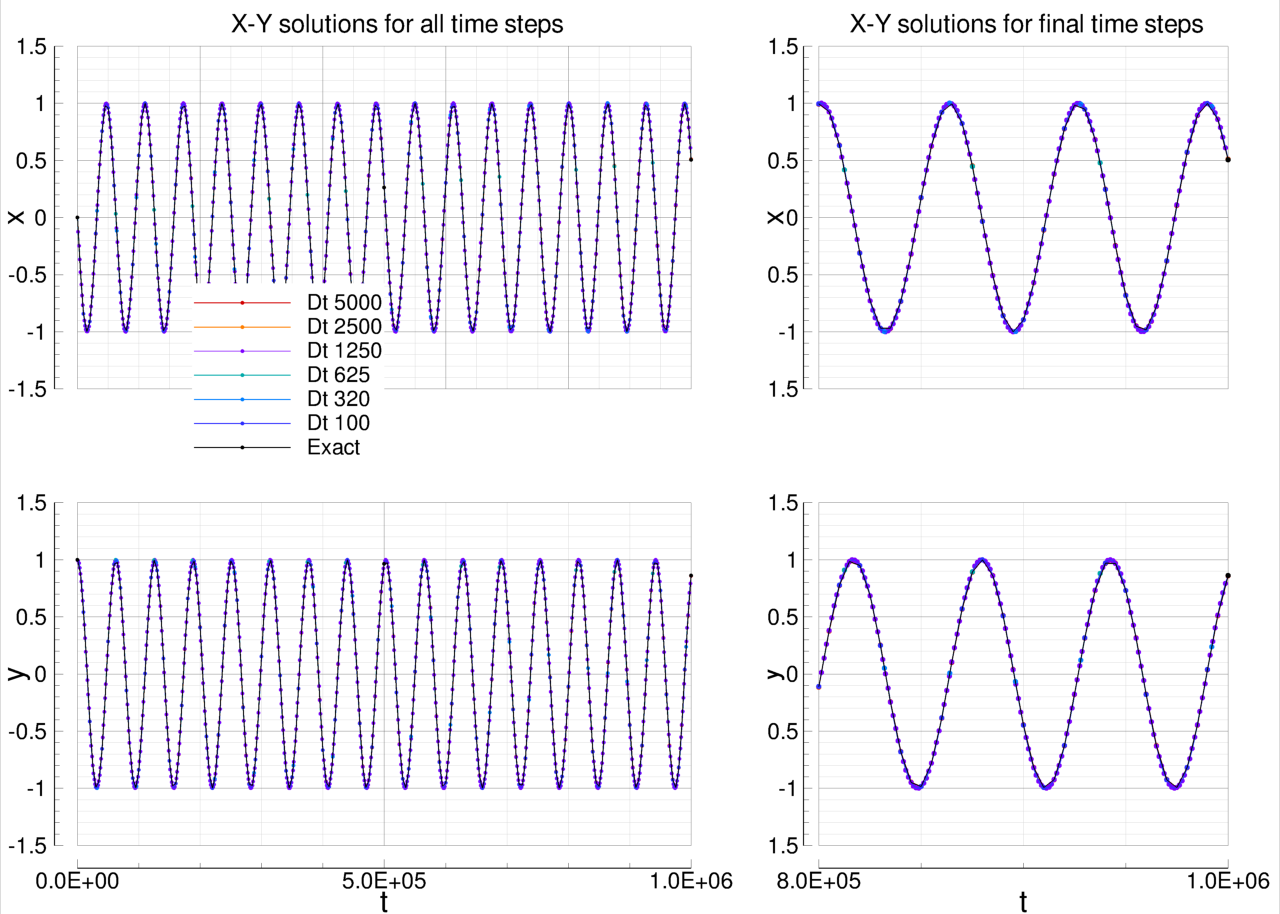
\includegraphics[width=1.00\textwidth]{errors-analysis/oscillation/errors_analysis-oscillation-ls-runge-kutta-7.png}
    \caption{7 stages}\label{fig:results-oscillation-ls-runge-kutta-7}
  \end{subfigure}
  \begin{subfigure}[b]{0.45\textwidth}
    \centering
    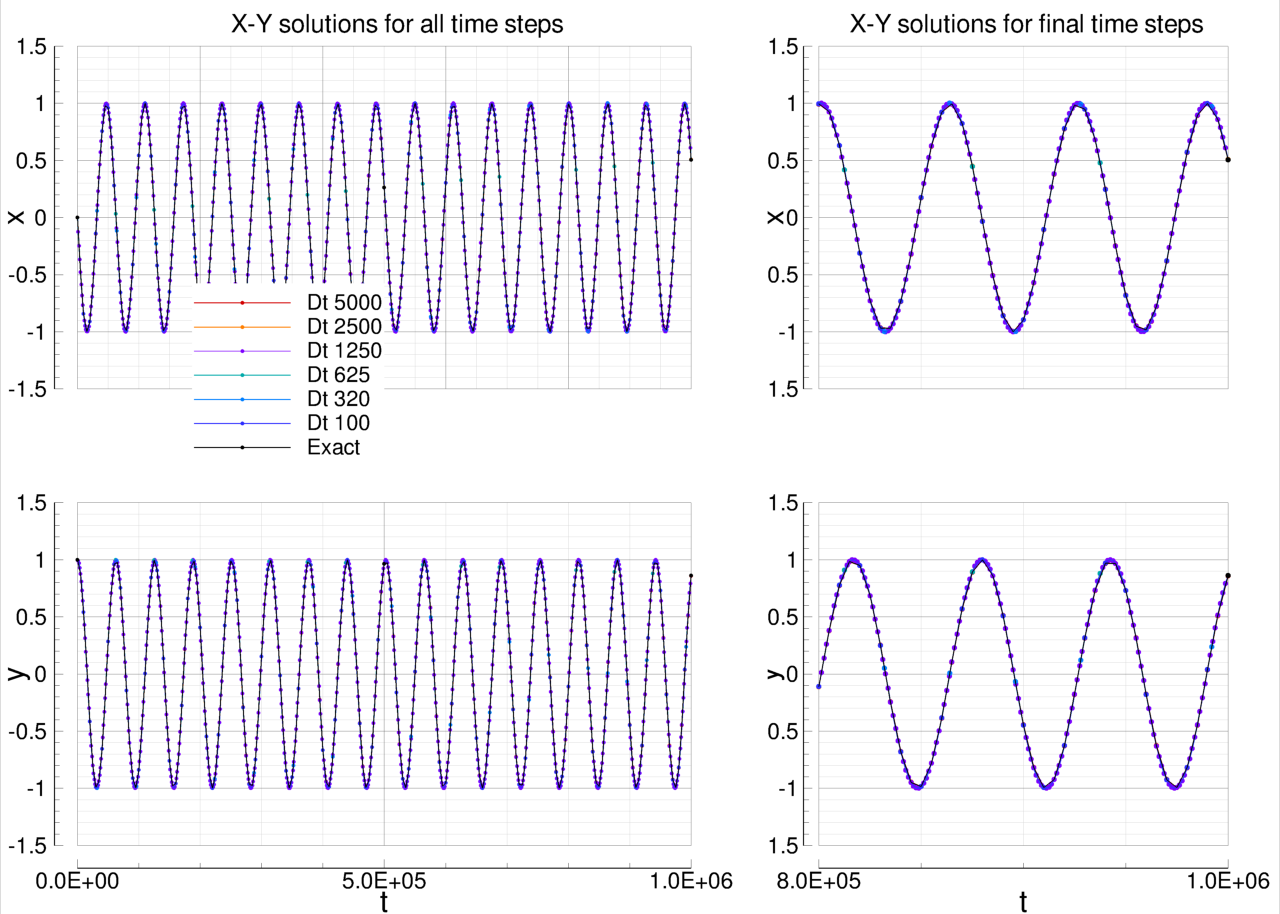
\includegraphics[width=1.00\textwidth]{errors-analysis/oscillation/errors_analysis-oscillation-ls-runge-kutta-12.png}
    \caption{12 stages}\label{fig:results-oscillation-ls-runge-kutta-12}
  \end{subfigure}\quad%
  \begin{subfigure}[b]{0.45\textwidth}
    \centering
    \includegraphics[width=1.00\textwidth]{errors-analysis/oscillation/errors_analysis-oscillation-ls-runge-kutta-13.png}
    \caption{13 stages}\label{fig:results-oscillation-ls-runge-kutta-13}
  \end{subfigure}
  \begin{subfigure}[b]{0.45\textwidth}
    \centering
    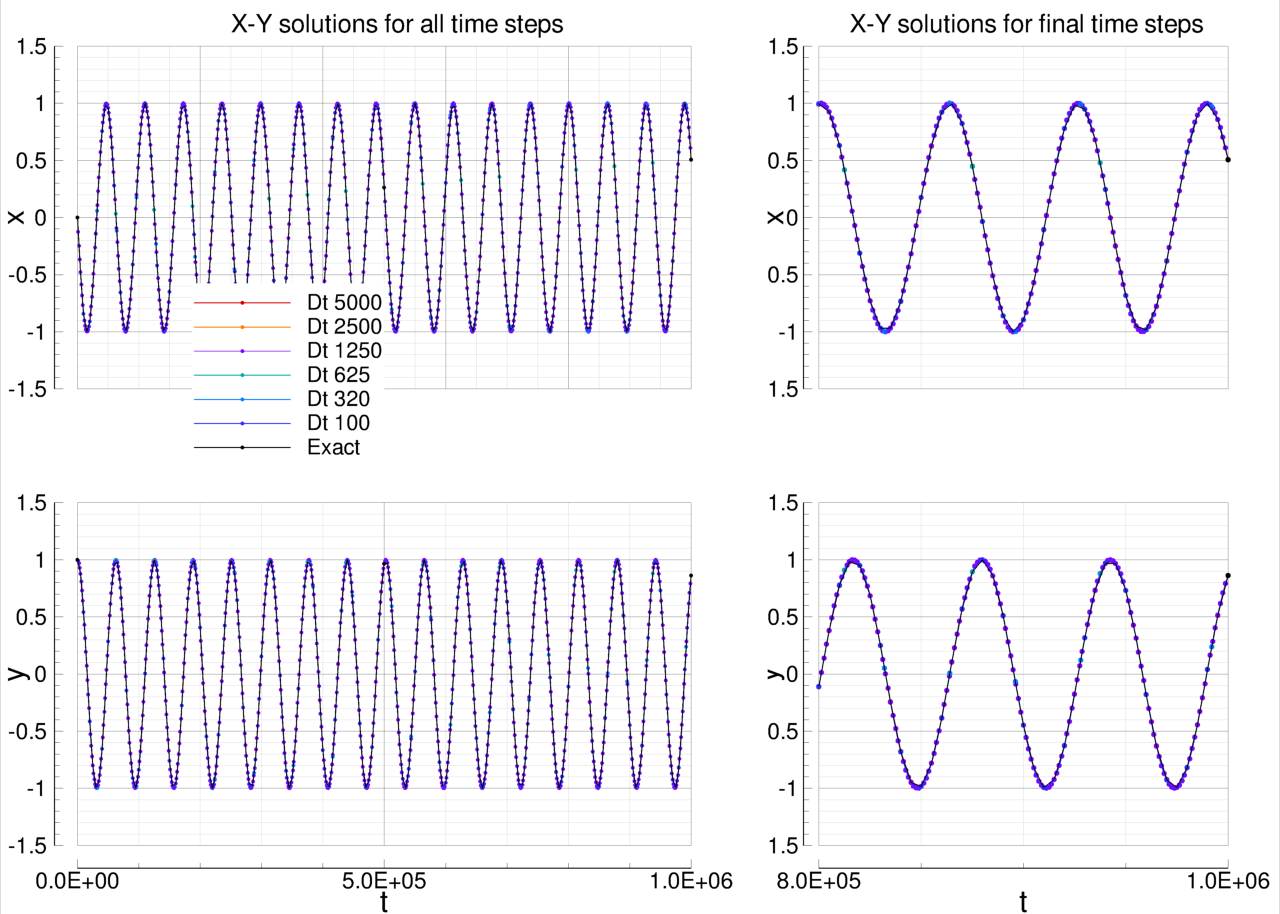
\includegraphics[width=1.00\textwidth]{errors-analysis/oscillation/errors_analysis-oscillation-ls-runge-kutta-14.png}
    \caption{14 stages}\label{fig:results-oscillation-ls-runge-kutta-14}
  \end{subfigure}\quad%
  \caption{Oscillation equations solutions computed by means of low storage Runge-Kutta solvers}\label{fig:results-oscillation-ls-runge-kutta-6-14}
\end{figure}



\subsubsection{TVD/SSP Runge-Kutta}

\begin{table}[!ht]
  \centering
  \caption{Oscillation test: errors analysis of explicit TVD/SSP Runge-Kutta}\label{tab:oscillation_errors_tvd_rk}
  \begin{subtable}[b]{0.40\textwidth}
    \centering
    \caption{1 stage}\label{tab:oscillation-tvd-rk-1}
    \resizebox{1.00\textwidth}{!}{%
    \begin{tabular}{ccccc}
      \toprule
      {\sc Time Step} & {\sc Error X} & {\sc Error Y} & {\sc Order X} & {\sc Order Y} \\
      \hline
      5000.0          &  0.840E+10    &  0.706E+10    & /             & /             \\
      2500.0          &  0.503E+06    &  0.570E+06    & 14.03         & 13.60         \\
      1250.0          &  0.289E+04    &  0.272E+04    &  7.45         &  7.71         \\
       625.0          &  0.239E+03    &  0.232E+03    &  3.59         &  3.55         \\
       320.0          &  0.737E+02    &  0.722E+02    &  1.76         &  1.74         \\
       100.0          &  0.250E+02    &  0.247E+02    &  0.93         &  0.92         \\
      \bottomrule
    \end{tabular}}
  \end{subtable}\quad%
  \begin{subtable}[b]{0.40\textwidth}
    \centering
    \caption{2 stages}\label{tab:oscillation-tvd-rk-2}
    \resizebox{1.00\textwidth}{!}{%
    \begin{tabular}{ccccc}
      \toprule
      {\sc Time Step} & {\sc Error X} & {\sc Error Y} & {\sc Order X} & {\sc Order Y} \\
      \hline
      5000.0          &  0.316E+02    &  0.319E+02    & /             & /             \\
      2500.0          &  0.892E+01    &  0.894E+01    & 1.83          & 1.84          \\
      1250.0          &  0.301E+01    &  0.305E+01    & 1.57          & 1.55          \\
       625.0          &  0.106E+01    &  0.107E+01    & 1.51          & 1.51          \\
       320.0          &  0.387E+00    &  0.392E+00    & 1.50          & 1.50          \\
       100.0          &  0.676E-01    &  0.685E-01    & 1.50          & 1.50          \\
      \bottomrule
    \end{tabular}}
  \end{subtable}\\
  \begin{subtable}[b]{0.40\textwidth}
    \centering
    \caption{3 stages}\label{tab:oscillation-tvd-rk-3}
    \resizebox{1.00\textwidth}{!}{%
    \begin{tabular}{ccccc}
      \toprule
      {\sc Time Step} & {\sc Error X} & {\sc Error Y} & {\sc Order X} & {\sc Order Y} \\
      \hline
      5000.0          &  0.255E+01    &  0.252E+01    & /             & /             \\
      2500.0          &  0.523E+00    &  0.516E+00    & 2.28          & 2.29          \\
      1250.0          &  0.944E-01    &  0.931E-01    & 2.47          & 2.47          \\
       625.0          &  0.167E-01    &  0.165E-01    & 2.50          & 2.50          \\
       320.0          &  0.314E-02    &  0.310E-02    & 2.50          & 2.50          \\
       100.0          &  0.171E-03    &  0.169E-03    & 2.50          & 2.50          \\
      \bottomrule
    \end{tabular}}
  \end{subtable}\quad%
  \begin{subtable}[b]{0.40\textwidth}
    \centering
    \caption{5 stages}\label{tab:oscillation-tvd-rk-5}
    \resizebox{1.00\textwidth}{!}{%
    \begin{tabular}{ccccc}
      \toprule
      {\sc Time Step} & {\sc Error X} & {\sc Error Y} & {\sc Order X} & {\sc Order Y} \\
      \hline
      5000.0          &  0.139E+00    &  0.141E+00    & /             & /             \\
      2500.0          &  0.122E-01    &  0.124E-01    & 3.50          & 3.50          \\
      1250.0          &  0.108E-02    &  0.110E-02    & 3.50          & 3.50          \\
       625.0          &  0.956E-04    &  0.969E-04    & 3.50          & 3.50          \\
       320.0          &  0.937E-05    &  0.949E-05    & 3.47          & 3.47          \\
       100.0          &  0.512E-06    &  0.519E-06    & 2.50          & 2.50          \\
      \bottomrule
    \end{tabular}}
  \end{subtable}
\end{table}

\begin{figure}[!ht]
  \centering
  \begin{subfigure}[b]{0.45\textwidth}
    \centering
    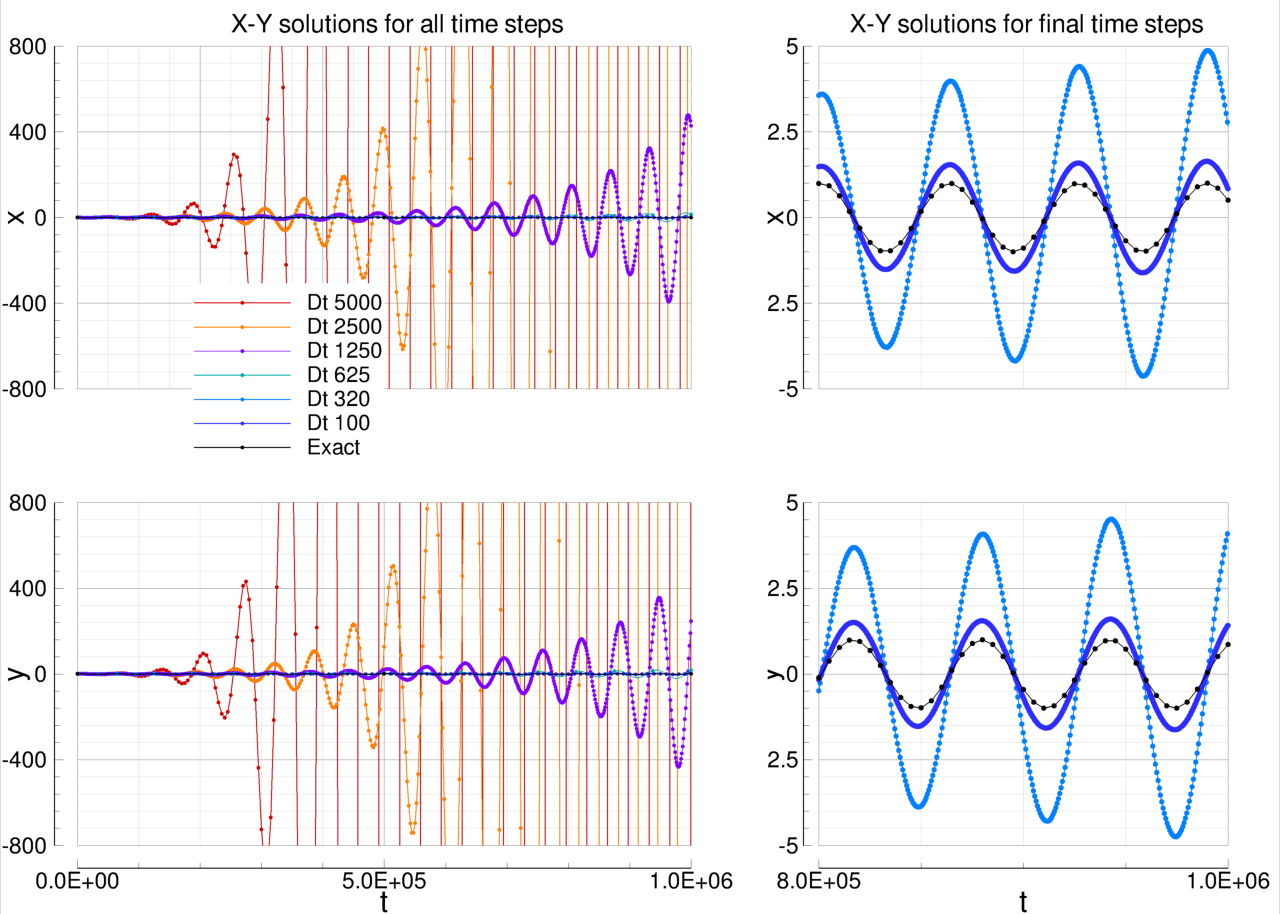
\includegraphics[width=1.00\textwidth]{errors-analysis/oscillation/errors_analysis-oscillation-tvd-runge-kutta-1.png}
    \caption{1 stage}\label{fig:results-oscillation-tvd-runge-kutta-1}
  \end{subfigure}\quad%
  \begin{subfigure}[b]{0.45\textwidth}
    \centering
    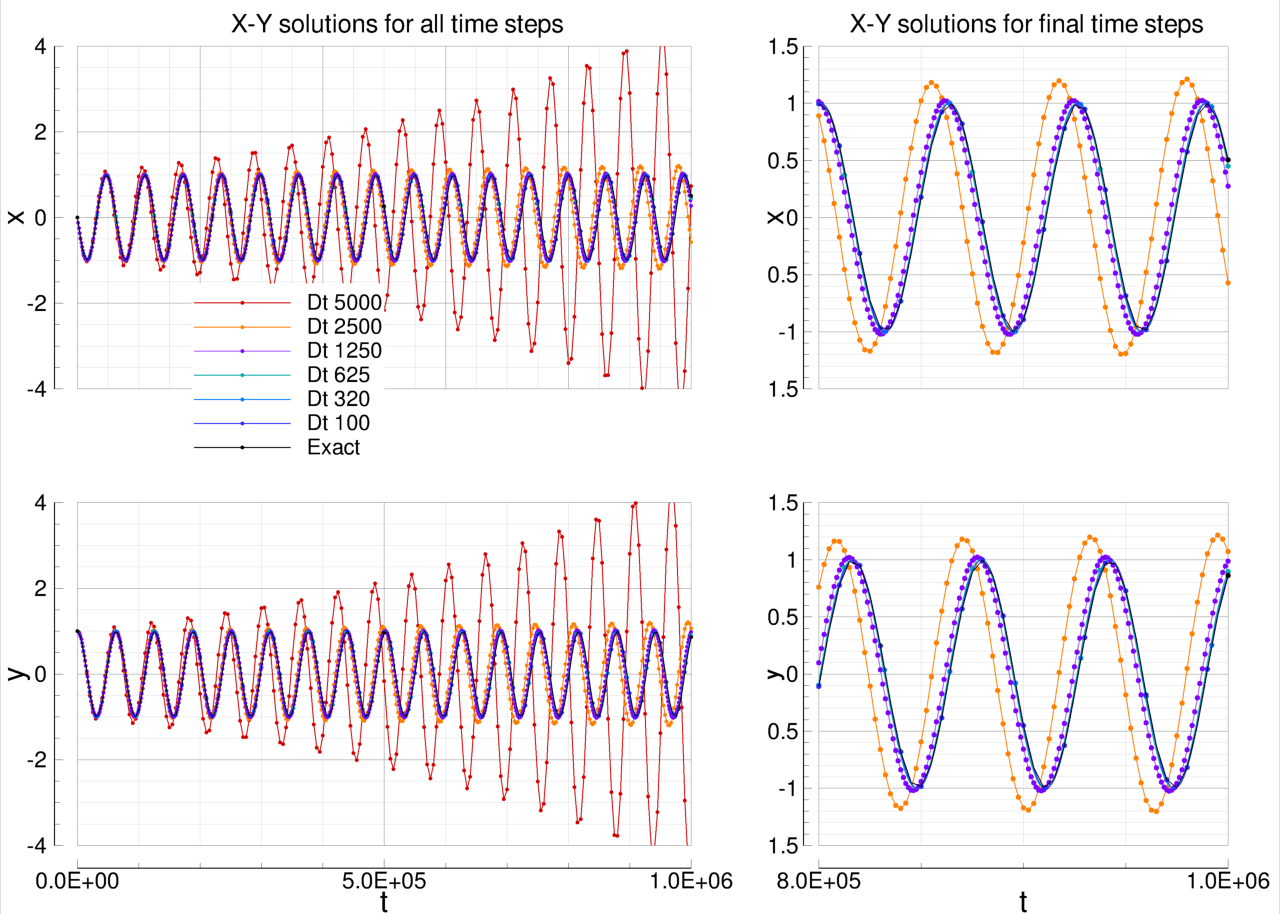
\includegraphics[width=1.00\textwidth]{errors-analysis/oscillation/errors_analysis-oscillation-tvd-runge-kutta-2.png}
    \caption{2 stages}\label{fig:results-oscillation-tvd-runge-kutta-2}
  \end{subfigure}\\
  \begin{subfigure}[b]{0.45\textwidth}
    \centering
    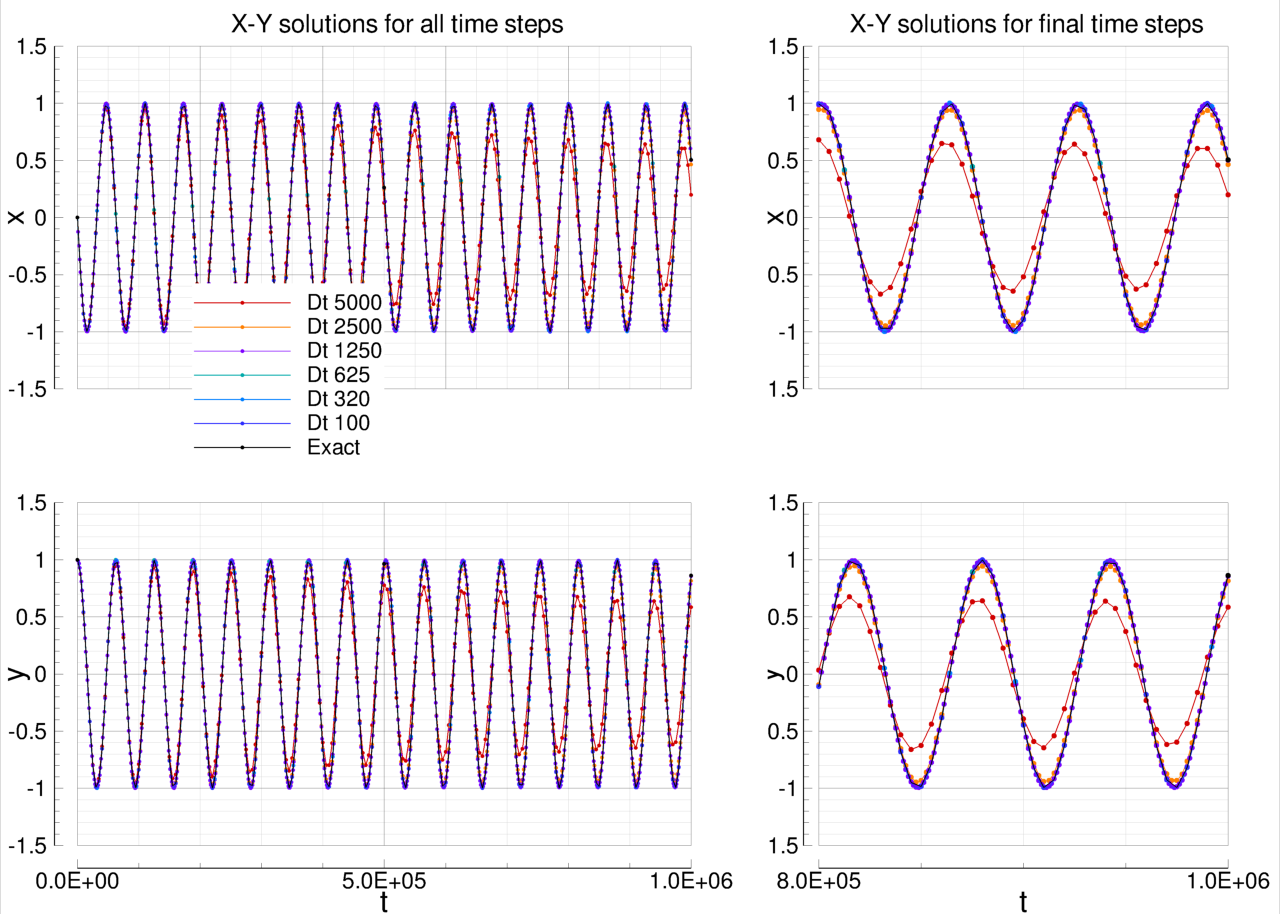
\includegraphics[width=1.00\textwidth]{errors-analysis/oscillation/errors_analysis-oscillation-tvd-runge-kutta-3.png}
    \caption{3 stages}\label{fig:results-oscillation-tvd-runge-kutta-3}
  \end{subfigure}\quad%
  \begin{subfigure}[b]{0.45\textwidth}
    \centering
    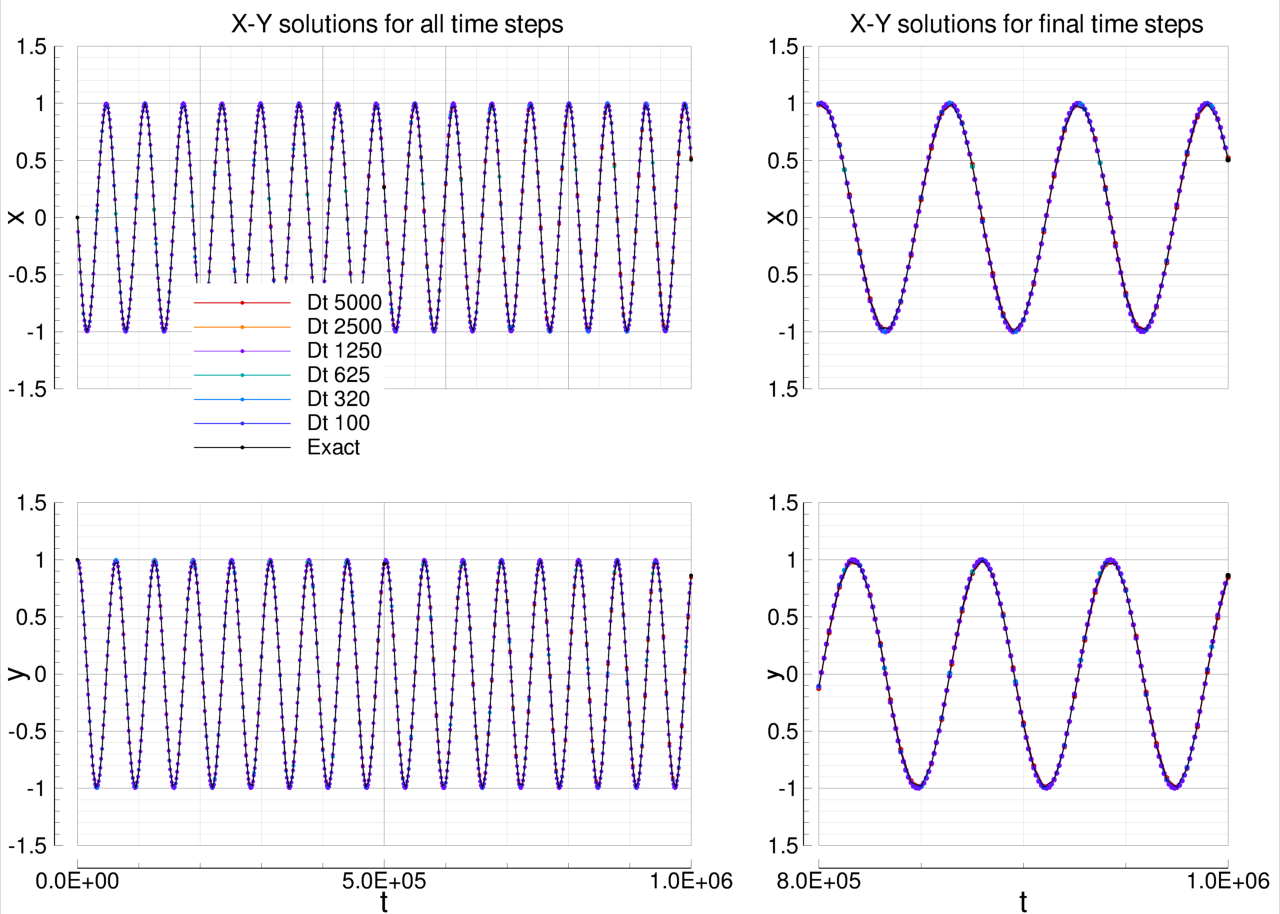
\includegraphics[width=1.00\textwidth]{errors-analysis/oscillation/errors_analysis-oscillation-tvd-runge-kutta-5.png}
    \caption{5 stages}\label{fig:results-oscillation-tvd-runge-kutta-5}
  \end{subfigure}\\
  \caption{Oscillation equations solutions computed by means of TVD/SSP Runge-Kutta solvers}\label{fig:results-oscillation-tvd-runge-kutta}
\end{figure}



\subsubsection{Embedded Runge-Kutta}

\begin{table}[!ht]
  \centering
  \caption{Oscillation test: errors analysis of explicit embedded Runge-Kutta solvers}\label{tab:oscillation_errors_emd_rk}
  \begin{subtable}[b]{0.40\textwidth}
    \centering
    \caption{7 stages}\label{tab:oscillation-emd-rk-7}
    \resizebox{1.00\textwidth}{!}{%
    \begin{tabular}{ccccc}
      \toprule
      {\sc Mean Time Step} & {\sc Error X} & {\sc Error Y} & {\sc Order X} & {\sc Order Y} \\
      \hline
      7352.9               &  0.626E-01    &  0.622E-01    & /             & /             \\
      3759.4               &  0.482E-02    &  0.480E-02    & 3.82          & 3.82          \\
      2272.7               &  0.793E-03    &  0.786E-03    & 3.59          & 3.59          \\
      1379.3               &  0.393E-04    &  0.390E-04    & 6.02          & 6.02          \\
       618.8               &  0.216E-05    &  0.213E-05    & 3.62          & 3.62          \\
       356.0               &  0.252E-06    &  0.249E-06    & 3.89          & 3.88          \\
      \bottomrule
    \end{tabular}}
  \end{subtable}\\
\end{table}

\begin{figure}[!ht]
  \centering
  \begin{subfigure}[b]{0.45\textwidth}
    \centering
    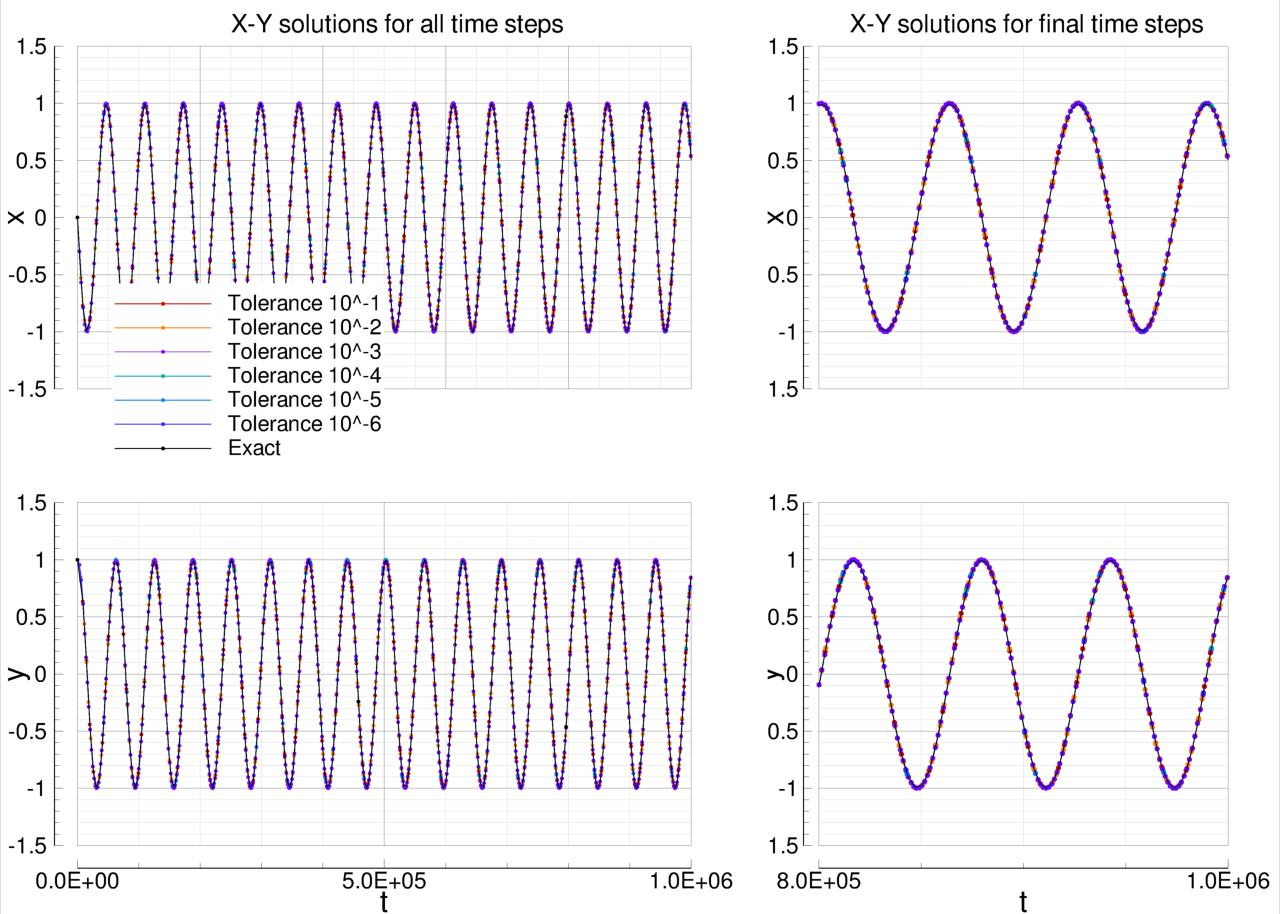
\includegraphics[width=1.00\textwidth]{errors-analysis/oscillation/errors_analysis-oscillation-emd-runge-kutta-7.png}
    \caption{7 stages}\label{fig:results-oscillation-emd-runge-kutta-7}
  \end{subfigure}\quad%
  \caption{Oscillation equations solutions computed by means of embedded Runge-Kutta solvers}\label{fig:results-oscillation-emd-runge-kutta-1-7}
\end{figure}

